
\documentclass[10pt,presentation,shownotes]{beamer}
\usetheme{Warsaw}

\usecolortheme{crane}

\usepackage{beamerthemesplit}
\usepackage{blindtext}
\usepackage{hyperref}
\usepackage{amsmath}
\usepackage{breqn}
\usepackage{alphabeta}

\usefonttheme{default}
\setbeamertemplate{caption}[numbered]
\setbeamercolor{block body example}{bg=green!12}
% \setbeamertemplate{navigation symbols}{}
% \setbeamercovered{transparent}

\setbeamertemplate{theorems}[numbered]

% Refer to these super useful links for beamer tips and tricks
%
% http://tug.ctan.org/macros/latex/contrib/beamer/doc/beameruserguide.pdf
% https://www.overleaf.com/learn/latex/Beamer

% THE FOLLOWING TEX FILE IS VERY CUSTOMISED SO IT IS RECOMMENDED YOU GO WITH SOME OTHER BEAMER TEMPLATE IF YOU WISH TO MAKE YOUR OWN CHANGES TO THE BEAMER SLIDE DESIGN.

\usepackage[utf8]{inputenc}
\usepackage[T1]{fontenc}
\usepackage{lmodern}
\usepackage[english]{babel}
\usepackage{csquotes}
\usepackage{mathtools,amsfonts,amssymb,tikz-cd,hyperref,caption,pstricks,setspace,booktabs,hyperref}
\usepackage{appendixnumberbeamer}
\usepackage{tikz}

%by me;
\usepackage{tikz}
\usepackage{pifont}
\usepackage{textpos}
\usepackage{pslatex}
%\usepackage[T1]{fontenc}
%\usepackage{mathptmx}
\usepackage{draftwatermark}
\usepackage[normalem]{ulem}
\usepackage{ragged2e}
\usepackage{amssymb}
\usepackage{bm}
\usepackage{fontawesome}

\newcommand\PlaceText[3]{%
\begin{tikzpicture}[remember picture,overlay]
\node[outer sep=0pt,inner sep=0pt,anchor=south west] 
  at ([xshift=#1,yshift=-#2]current page.north west) {#3};
\end{tikzpicture}%
}


%%%%%%%%%%%%%%%%%%%%%%%%%%%%%%%%%%%%%%%%%%%%%%%%%%%%%%%%%%%%%%%%%%%%%%%%%%%%%%%%%%
% Customize hyperlink colours
\usepackage{xcolor}
\hypersetup{
	colorlinks,
	linkcolor={blue!50!black},
	citecolor={blue!50!black},
	urlcolor={blue!80!black}
}

% We use BiBLaTeX for our bibliography.
\usepackage[backend=biber,style=alphabetic]{biblatex}
\renewcommand*{\nameyeardelim}{\addcomma\addspace}

\addbibresource{References/ref.bib}

% The lipsum package called in the next line is just for generating dummy text and is not necessary.
\usepackage{lipsum}

% Note: Changes to specific presentation elements usually start with /makeatletter and ends with /makeatother

\makeatletter
\def\th@remark{%
    \normalfont % body font
    \setbeamercolor{block title example}{bg=orange,fg=black}
    \setbeamercolor{block body example}{bg=orange!20,fg=black}
    \def\inserttheoremblockenv{exampleblock}
  }
\makeatother

\theoremstyle{remark}
\newtheorem*{remark}{Remark}

\setbeamertemplate{headline}
{
  \leavevmode%
  \hbox{%
  \begin{beamercolorbox}[wd=.5\paperwidth,ht=2.5ex,dp=1ex,left,leftskip=1em]{section in head/foot}%
    \usebeamerfont{subsection in head/foot}\hspace*{2ex}\insertshorttitle
  \end{beamercolorbox}%
  \begin{beamercolorbox}[wd=.5\paperwidth,ht=2.5ex,dp=1ex,center]{date in head/foot}%
    \usebeamerfont{date in head/foot}\insertshortdate{}\hspace*{2ex}
  \end{beamercolorbox}}%
  \vskip0pt%
}

\makeatletter
\setbeamertemplate{footline}
{
  \leavevmode%
  \hbox{%
  \begin{beamercolorbox}[wd=.33\paperwidth,ht=2.25ex,dp=1ex,center]{author in head/foot}%
    \usebeamerfont{author in head/foot}\insertshortauthor~~\beamer@ifempty{\insertshortinstitute}{}{(\insertshortinstitute)}
  \end{beamercolorbox}%
  \begin{beamercolorbox}[wd=.34\paperwidth,ht=2.25ex,dp=1ex,center]{subsection in head/foot}%
    \usebeamerfont{section in head/foot}\hspace*{1ex}\insertsectionhead\hspace*{1ex}
  \end{beamercolorbox}%
  \begin{beamercolorbox}[wd=.33\paperwidth,ht=2.25ex,dp=1ex,right, rightskip=1em]{section in head/foot}%
    \usebeamerfont{section in head/foot}\insertsubsectionhead\hspace*{2ex}
  \end{beamercolorbox}}%
  \vskip0pt%
}
\makeatother

\makeatletter
\setbeamertemplate{frametitle}{
    \ifbeamercolorempty[bg]{frametitle}{}{\nointerlineskip}%
    \@tempdima=\textwidth%
    \advance\@tempdima by\beamer@leftmargin%
    \advance\@tempdima by\beamer@rightmargin%
    \begin{beamercolorbox}[sep=0.3cm,center,wd=\the\@tempdima]{frametitle}
        \usebeamerfont{frametitle}%
        \vbox{}\vskip-1ex%
        \if@tempswa\else\csname beamer@ftecenter\endcsname\fi%
        \strut\insertframetitle\strut\par%
        {%
            \ifx\insertframesubtitle\@empty%
            \else%
            {\usebeamerfont{framesubtitle}\usebeamercolor[fg]{framesubtitle}\insertframesubtitle\strut\par}%
            \fi
        }%
        \vskip-1ex%
        \if@tempswa\else\vskip-.3cm\fi% set inside beamercolorbox... evil here...
    \end{beamercolorbox}%
}
\makeatother

% This code displays an updating ToC at the beginning of every section.
\AtBeginSection[]
{
	\begin{frame}
	\frametitle{Table of Contents}
	\tableofcontents[currentsection]
	\end{frame}
}

\makeatletter
\newcommand<>{\insertsubsectiontitle}{\frametitle{\insertsubsection}}
\let\oldbeamer@checkframetitle\beamer@checkframetitle% Store the \frametitle checking mechanism
\renewcommand<>{\subsection}{%
  \gdef\beamer@checkframetitle{% Update \frametitle checking to ...
    \insertsubsectiontitle% ...insert the section title and...
    \global\let\beamer@checkframetitle\oldbeamer@checkframetitle% ...revert to it's old definition
  }% Regular \section stuff follows
  \alt#1{\@ifnextchar[\beamer@subsection\beamer@@subsection}
    {\beamer@secgobble}}
\makeatother

\makeatletter
\newenvironment<>{proofs}[1][\proofname]{%
    \par
    \def\insertproofname{#1\@addpunct{.}}%
    \usebeamertemplate{proof begin}#2}
  {\usebeamertemplate{proof end}}
\makeatother

% Uncomment for some standard notations in math (Real, Complex and Rational numbers, Norm, Jacobian, etc) 
% \newcommand{\reals}{\mathbb{R}}
% \newcommand{\mtrx}{\mathbb{M}}
% \newcommand{\jacobian}{\mathcal{J}}
% \newcommand{\tallstrut}{\vphantom{\frac{5_A}{4,10^3}}}
% \newcommand{\abs}[1]{\left\lvert #1 \right\rvert}
% \newcommand{\norm}[1]{\left\lVert #1 \right\rVert}

%inceputul doc. oficial

%PRIMA PAGINA;

% Extended input for Title Page, Abridged Input for Header and Footer
\title[\color{black} Prezentare Practica IF - 2022

\hspace{0.3cm}\insertframenumber/\inserttotalframenumber]{\textbf{Aplicații în fizica energiilor înalte- HEP}}

%autor + sup.
\author[Andreicovici Iulian Florin]{{\textit{\textbf{Student:} Andreicovici Iulian Florin}
{\and} \\
{\textit{}} \\
{\textbf{Tutore:} Andrei Geantă} \\ {\textbf{Profesor Coordonator:}} Neguțu Constantin}}

%\usepackage{setspace}\onehalfspace

\institute[UPB]{\textbf{UPB - Universitatea POLITEHNICA din București }}

\date[Short Presentation Details]{\underline{Idei și inițiative generale - specifice aplicațiilor din aria HEP.}}
\date{\textbf{Data:} 12.09.2022}
\titlegraphic{
\includegraphics[height=50pt]{Logos and Figures/upb_logo_200ani_v1-289x300.png}}


\begin{document}

\setlength{\belowcaptionskip}{10pt plus 2pt minus 4pt}	
	
 \begin{frame}[plain]
		\maketitle
	\end{frame}



%sectiunea1.............................................................................................................
\section{\textbf{Scopul și motivația.}}


%slide1(ce mi-am propus)
 \begin{frame}{\textbf{Ce mi-am propus să fac și ce m-a motivat}}
 
 \vspace{-0.25cm}
   \makebox[0.7cm]{} \textit{Evident...}  \textit{\textbf{motivația mea principală}} atunci când am ales această direcție de studiu a fost centrată pe necesitatea însușirii unui set de noi competențe în materie de \textit{ fizică nucleară și programare}.

 \vspace{0.5cm}
  \textit{\textbf{\dashuline{Mi-am propus să abordez două teme generale de studiu;}}}

  \begin{enumerate} 
    
       \item[$\blacksquare$] \makebox[0.5cm]{} \textit{\textbf{Detectarea particulelor elementare în cadrul proiectului ATLAS} - LHC prin plotarea și interpretarea datelor experimentale cu ajutorul aplicației soft \textbf{HYPATIA} - izolarea bosonilor de etalonare.}
       
       \item[$\blacksquare$] \makebox[0.5cm]{} \textit{\textbf{Instalarea și utilizarea pachetului GEANT4} - programarea unor aplicații de simulare interactivă a detectorilor de radiație:}
       
    \begin{enumerate}  
        \item \textcolor{blue} {detectorul cu Ge hiperpur - HPGe.}
        \item \textcolor{green} {detectorul de radiație Cherenkov.}
        \item \textcolor{red} {simularea radiației cosmice în atmosferă - jet atmosferic.}
        
     \end{enumerate}

 
 \end{enumerate}

 \end{frame}

 
%slide2(ce m-a motivat)
% \begin{frame}{\textbf{Motivația – de ce am ales subiectul?}}
 
 %\end{frame}



%secțiunea2;

\section{\textbf{Activități propuse.}}

%frame 1 - ce activitati am stabilit
 \begin{frame}{\textbf{Lista activităților stabilite convențional}}
 
\vspace{0cm}
  \textit{\textbf{\makebox[0.5cm]{} Activitățile propuse au la bază demararea acțiunii asupra căreia s-au focalizat obiectivele majore;}}

  \begin{itemize}
    
      \item[\ding{43}]  \makebox[0.5cm]{} \textcolor{violet}{\textbf{Instalarea suportului software necesar rulării aplicațiilor: SO LINUX + HYPATIA și GEANT4. }}
      
     \item[\ding{235}]  \makebox[0.5cm]{} \textcolor{violet}{\textbf{Crearea unor prezentări introductive despre subiectele abordate în LaTeX și Office: Word + PowerPoint(studii generale de caz).}}
     
     \item[\ding{52}]  \makebox[0.5cm]{} \textcolor{violet}{\textbf{Analiza fizică specifică modului de funcționare al proiectului ATLAS-LHC: detectarea bosonilor de etalonare prin procesarea datelor evenimentelor reale cu ajutorul tools-ului HYPATIA.}}
     
     \item[\ding{227}] \makebox[0.5cm]{} \textcolor{violet}{\textbf{Simularea unor detectori de radiație cu ajutorul pachetului GEANT4: rularea, prezentarea, înțelegerea, programarea și depanarea unor aplicații în limbajul C++(paradigma OOP)! }}
        
 \end{itemize} 

 

 \end{frame}



%sectiunea3;
\section{\textbf{Instituția gazdă.}}

%frame 1 - ce activitati am stabilit
 \begin{frame}{\textbf{Instituția în cadrul căreia am efectuat stagiul de practică}}

 \vspace{0cm}
 \normalsize \textit{A) Activitatea de practică desfășurată în decursul verii a fost posibilă în urma parteneriatului cu:}
  \\

  \begin{center}
    \large  \textbf{\textit{-Institutul Național de CD în Fizică și Inginerie Nucleară "Horia Hulubei", IFIN-HH}}
  \end{center}

\vspace{1cm}  
\textit{\textcolor{red}{B) Departamentul de operare:}}

\begin{center}
    \large  \textbf{\textit{Departamentul de Fizica Particulelor Elementare (DFPE).}}
\end{center}

  
 
 \end{frame}



%sectiunea4;
\section{\textbf{Rezultate obținute}}

%frame1
\begin{frame}{\textbf{Rezultatele obținute corelate cu activitățile propuse}}


\vspace{-1.9cm}

\textit{\textbf{\makebox[0.5cm]{} Activitățile de bază au fost repartizate în funcție de săptămânile alocate astfel:}}\\


\vspace{0.5cm}
\textbf{\href{https://drive.google.com/drive/folders/107J5h6S5zOi1gQwBr6cD2lAjOTgSOvLS}{I) În prima săptămână (click):}}\\

\makebox[0.5cm]{}a) Instalarea și utilizarea sistemului de operare UBUNTU(LINUX).\\
\makebox[0.5cm]{}b) Însușirea bazelor limbajului LaTeX (partea de redactare/design).\\
\makebox[0.5cm]{}c) Crearea câtorva programe în Python pentru redarea efectelor relativiste necesare în HEP.\\

%latex img
\begin{tikzpicture}[overlay, remember picture]
\node[anchor=center, 
      xshift=-3cm, 
      yshift=-1.5cm] 
     at (current page.center) 
     {
\includegraphics[scale=0.1]{Chapters/LaTeX_project_logo_bird.svg.png}};
\end{tikzpicture}

%python
\begin{tikzpicture}[overlay, remember picture]
\node[anchor=center, 
      xshift=0cm, 
      yshift=-3cm] 
     at (current page.center) 
     {
\includegraphics[scale=0.05]{Chapters/Python_logo_and_wordmark.svg.png}};
\end{tikzpicture}


%Ubuntu
\begin{tikzpicture}[overlay, remember picture]
\node[anchor=center, 
      xshift=3cm, 
      yshift=-1.5cm] 
     at (current page.center) 
     {
\includegraphics[scale=0.09]{Chapters/maxresdefault.jpg}};
\end{tikzpicture}
 
\end{frame}

%program1

\begin{frame}

    %lorentz contraction
\begin{tikzpicture}[overlay, remember picture]
\node[anchor=center, 
      xshift=0cm, 
      yshift=-2cm] 
     at (current page.center) 
     {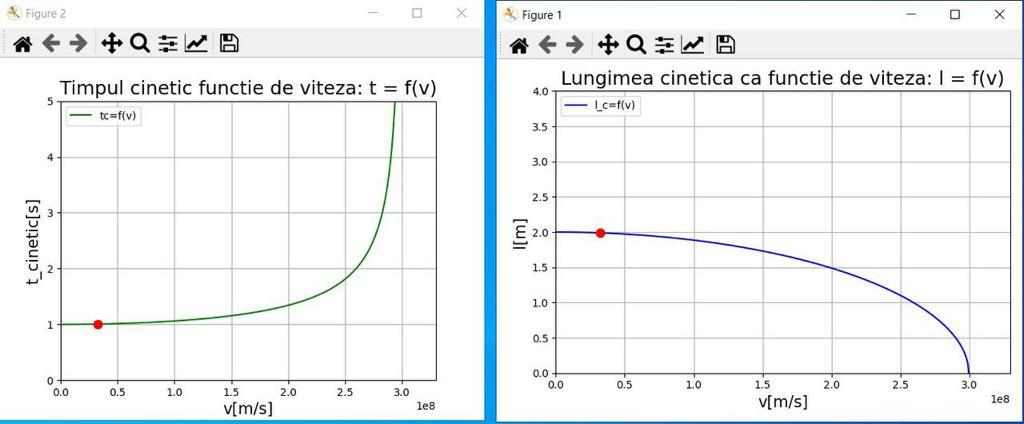
\includegraphics[scale=0.22]{Chapters/RezultatDep.jpeg}};
\end{tikzpicture}

  %RezGracifc
\begin{tikzpicture}[overlay, remember picture]
\node[anchor=center, 
      xshift=-3.5cm, 
      yshift=2cm] 
     at (current page.center) 
     {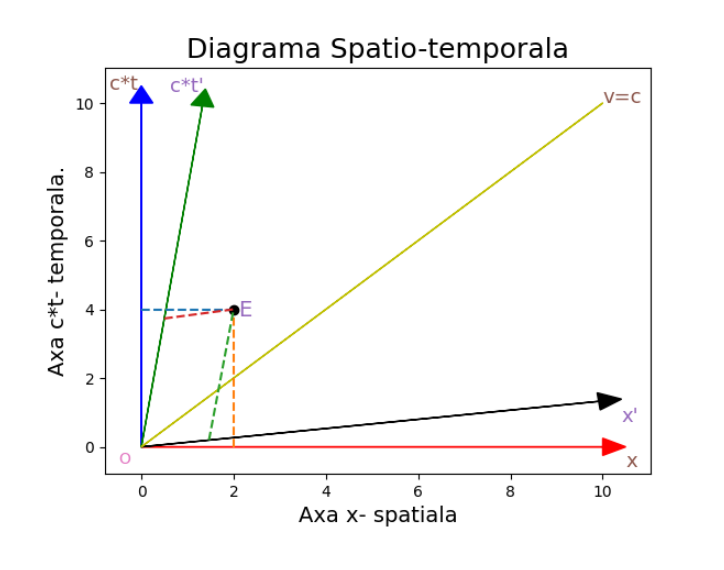
\includegraphics[scale=0.25]{Chapters/Rezultat_Diagrama.png}};
\end{tikzpicture}

\begin{tikzpicture}[overlay, remember picture]
\node[anchor=center, 
      xshift=2.7cm, 
      yshift=2cm] 
     at (current page.center) 
     {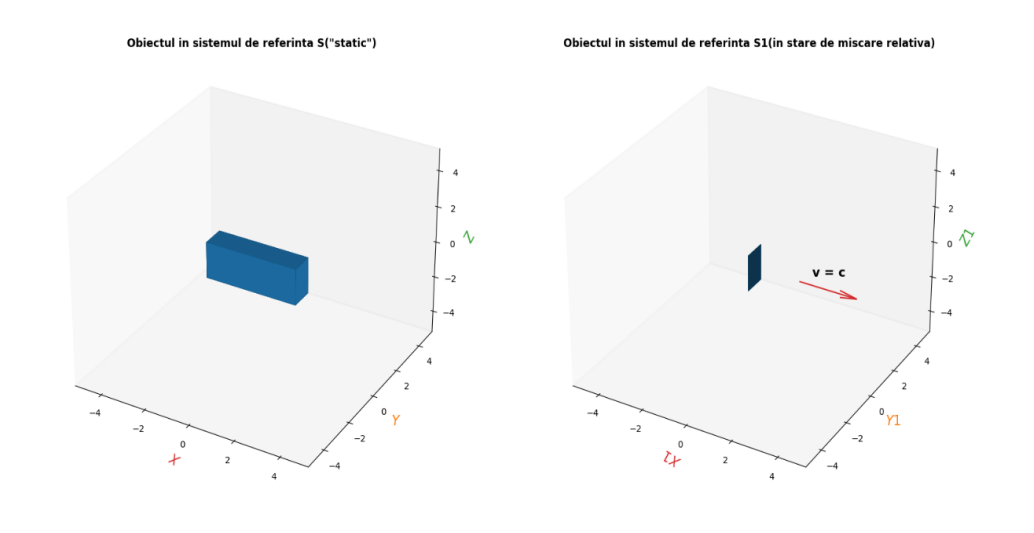
\includegraphics[scale=0.3]{Chapters/RezultatGraficIlustrat.png}};
\end{tikzpicture}


\end{frame}

%ubuntu desktop
\begin{frame}{}

\begin{tikzpicture}[overlay, remember picture]
\node[anchor=center, 
      xshift=0cm, 
      yshift=0cm] 
     at (current page.center) 
     {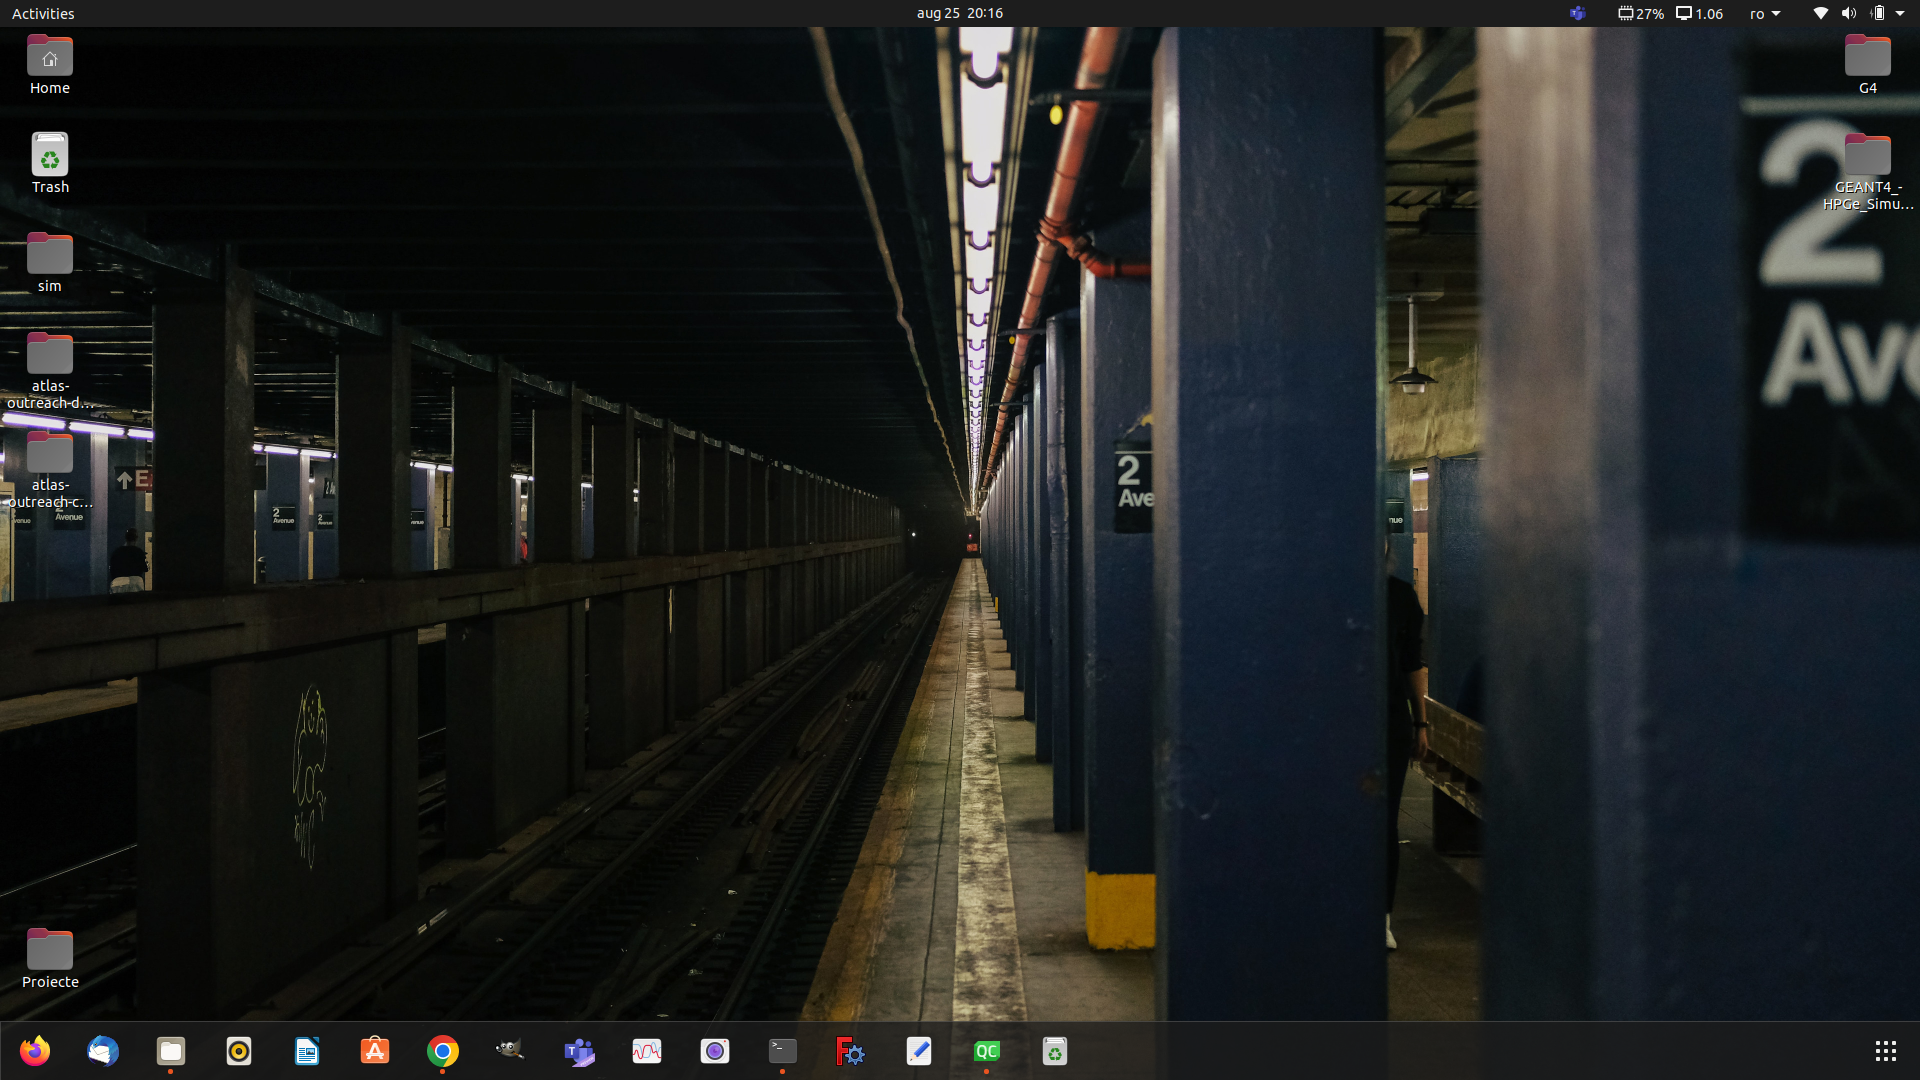
\includegraphics[scale=0.18]{Chapters/MyUbuntu_Desktop.png}};
\end{tikzpicture}


\end{frame}



\begin{frame}{}

\vspace{-3cm}

\textbf{\href{https://drive.google.com/drive/folders/1SHvtm29cUzZkMwOQRteytd-pLCQuIolb}{II) A doua săptămână (click):}}\\
\makebox[0.5cm]{}a) Clasificarea particulelor elementare - noțiuni teoretice de FP.\\
\makebox[0.5cm]{}b) Instalarea și utilizarea softului HYPATIA pentru analiza unor evenimente ATLAS.\\
\makebox[0.5cm]{}c) Conceptualizarea resurselor necesare detectării particulelor elementare - trecerea la partea experimentală.\\

%Ubuntu
\begin{tikzpicture}[overlay, remember picture]
\node[anchor=center, 
      xshift=-3cm, 
      yshift=-0.5cm] 
     at (current page.center) 
     {
\includegraphics[scale=0.15]{Chapters/Hypatia_Logo_800.jpg}};
\end{tikzpicture}

%Ubuntu
\begin{tikzpicture}[overlay, remember picture]
\node[anchor=center, 
      xshift=3.0cm, 
      yshift=-1.5cm] 
     at (current page.center) 
     {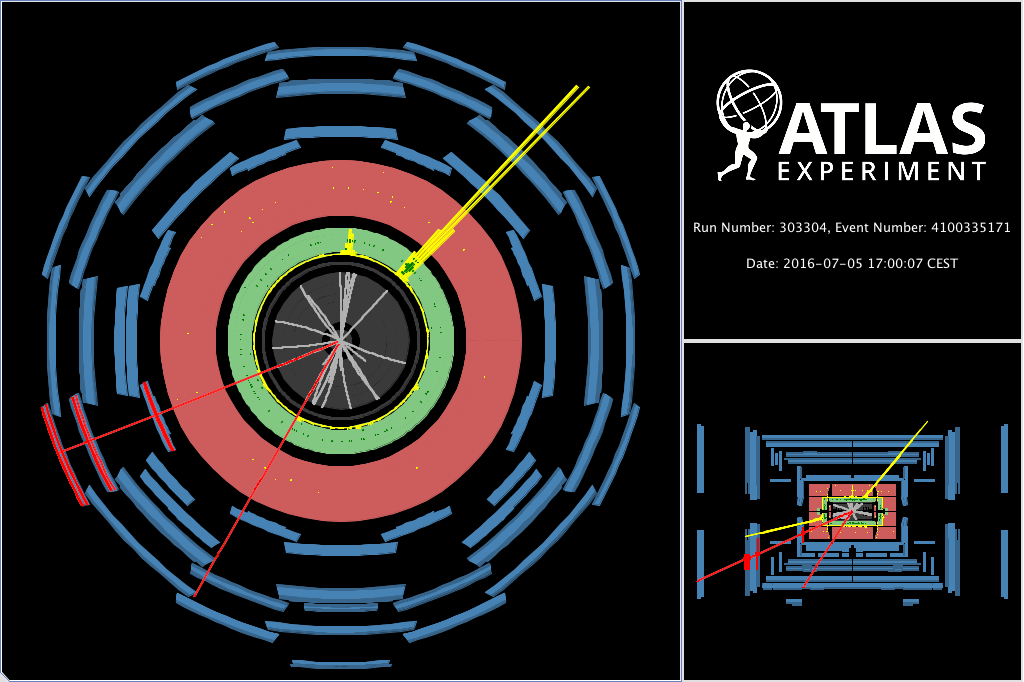
\includegraphics[scale=0.15]{Chapters/Particle-Physics.png}};
\end{tikzpicture}

\begin{tikzpicture}[overlay, remember picture]
\node[anchor=center, 
      xshift=-3.5cm, 
      yshift=-3cm] 
     at (current page.center) 
     {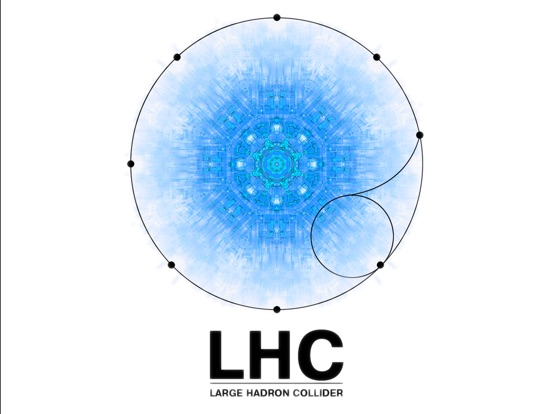
\includegraphics[scale=0.15]{Chapters/ATLAS.jpg}};
\end{tikzpicture}

\end{frame}


%standard model
\begin{frame}
    
\begin{tikzpicture}[overlay, remember picture]
\node[anchor=center, 
      xshift=0cm, 
      yshift=0cm] 
     at (current page.center) 
     {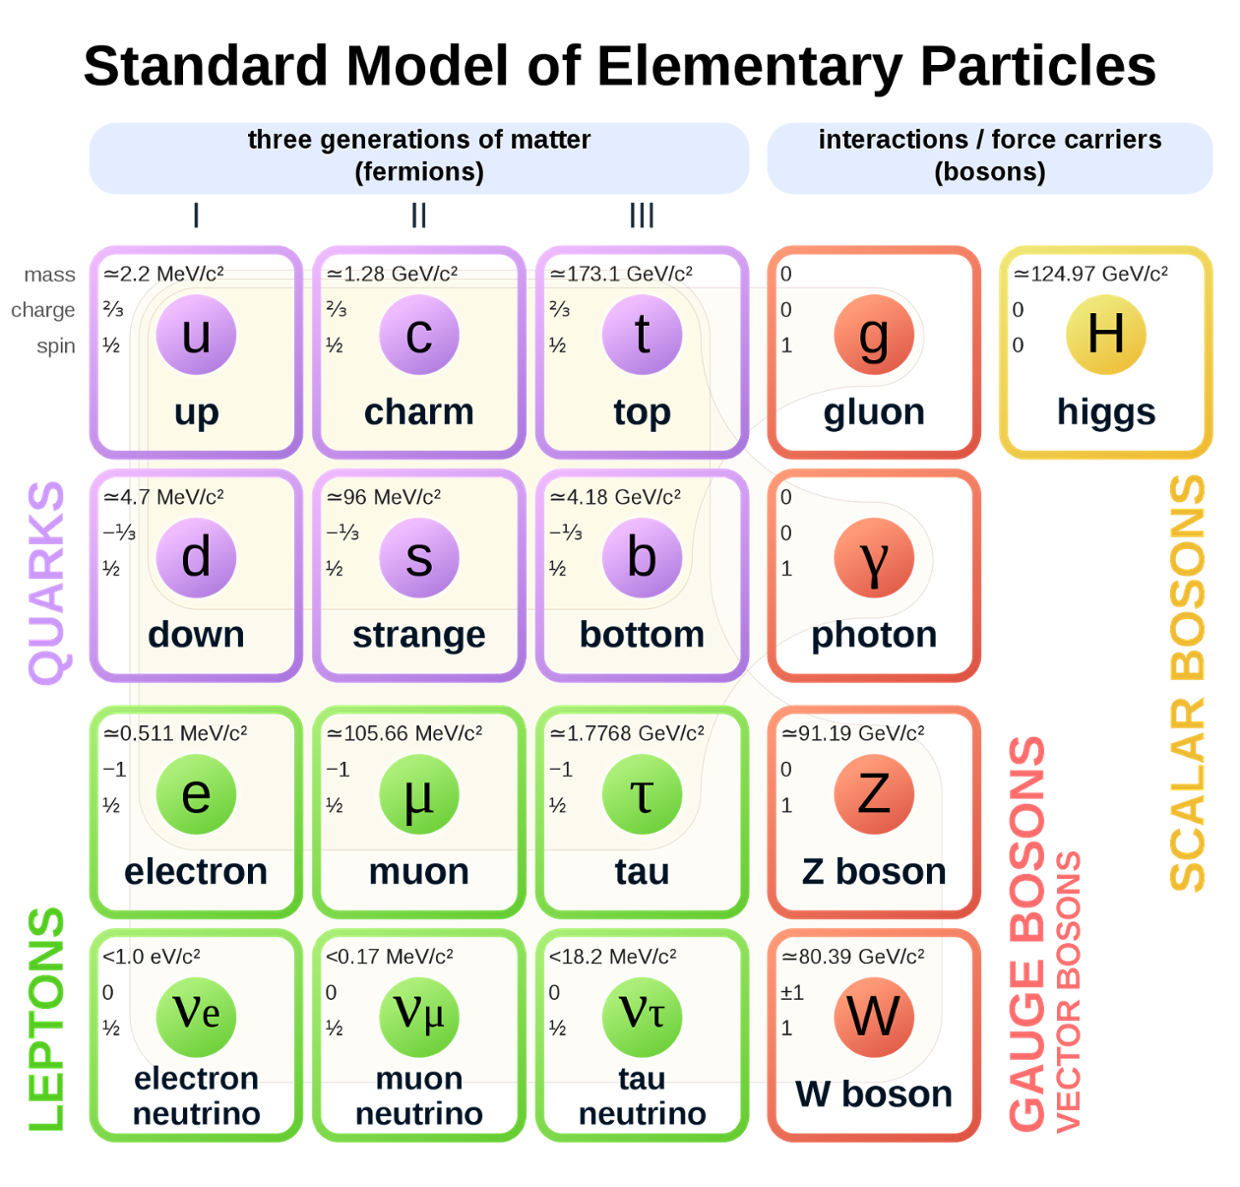
\includegraphics[scale=0.2]{Chapters/StandardModel.png}};
\end{tikzpicture}

\end{frame}


%saptamana 3
\begin{frame}{}

\vspace{-2.5cm}

\textbf{\href{https://drive.google.com/drive/folders/1oLQUEtq2emEDEpTa4WO_8CLfNnXbXhDh}{III) A treia săptămână (click):}}\\
\makebox[0.5cm]{}a) Detalierea ingineriei din spatele componentelor detectorului ATLAS de la LHC.\\
\makebox[0.5cm]{}b) Examinarea mecanismelor de izolare și evidențiere a particulelor elementare - izolarea tracks-urilor specifice unor bosoni de etalonare(W și Z).\\
\makebox[0.5cm]{}c) Teoretizarea modului de reconstruire efectivă a evenimentelor fizice de la ATLAS - distingerea canalelor de dezintegrare.\\

%Ubuntu
\begin{tikzpicture}[overlay, remember picture]
\node[anchor=center, 
      xshift=-2cm, 
      yshift=-1cm] 
     at (current page.center) 
     {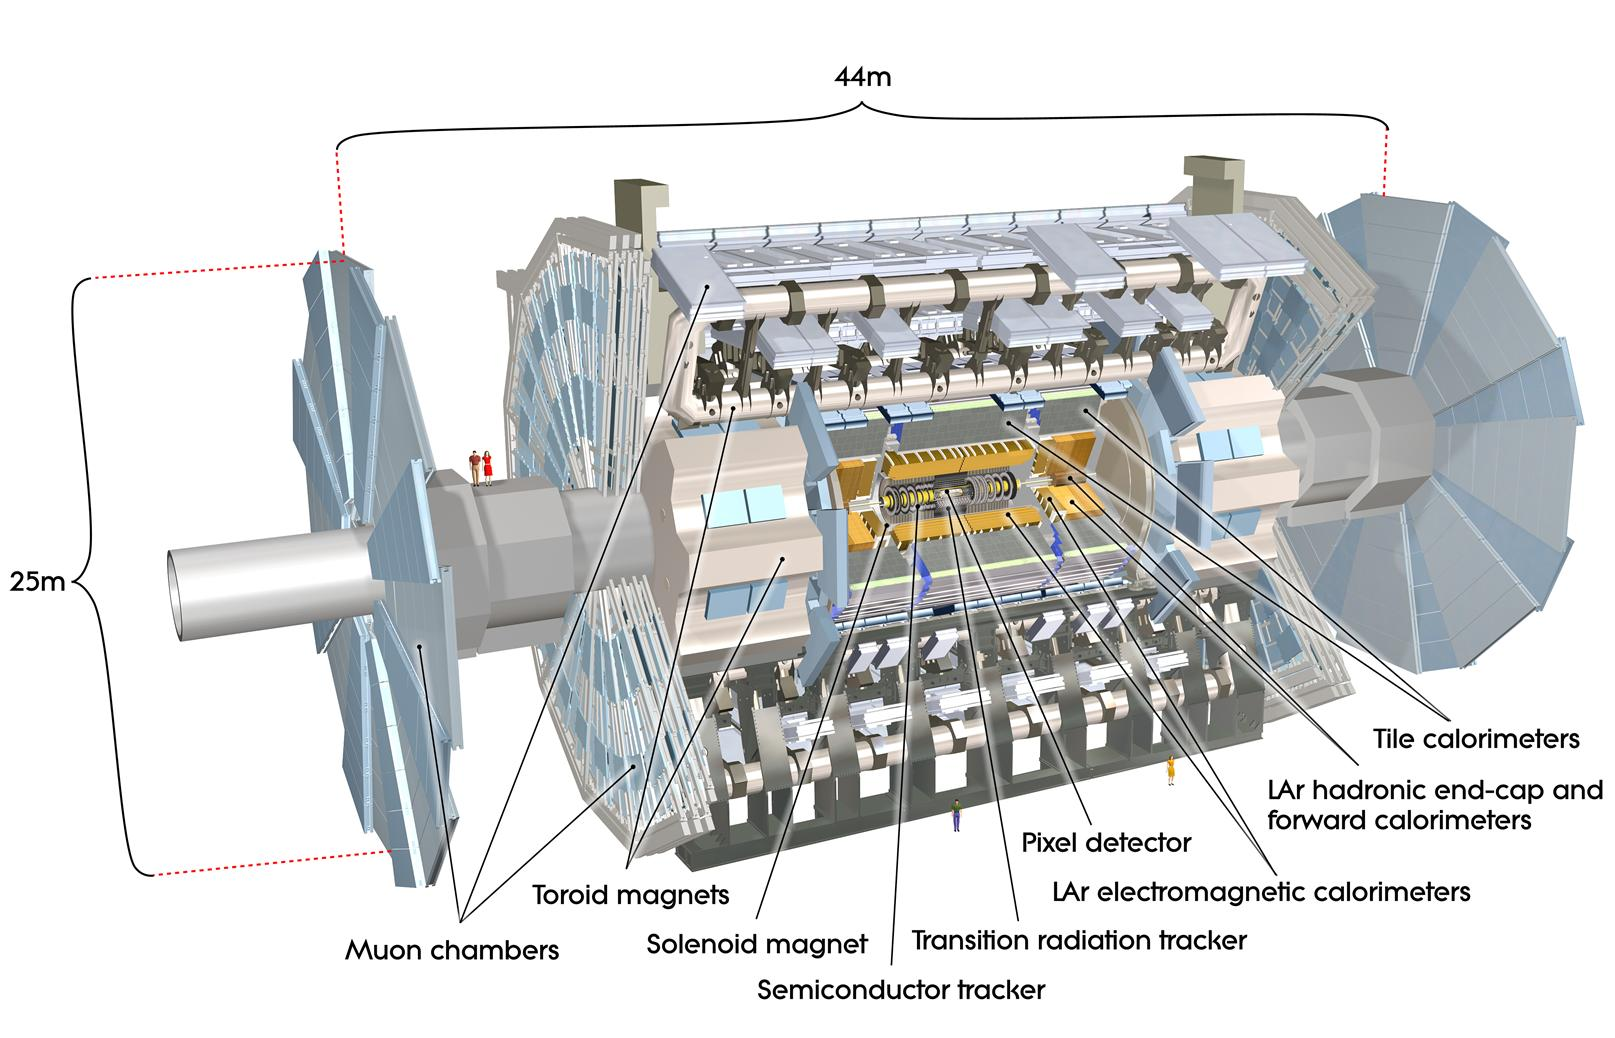
\includegraphics[scale=0.2]{Chapters/Mecanismul.jpg}};
\end{tikzpicture}

%Ubuntu
\begin{tikzpicture}[overlay, remember picture]
\node[anchor=center, 
      xshift=3.5cm, 
      yshift=-0.5cm] 
     at (current page.center) 
     {
\includegraphics[scale=0.05]{Chapters/cern.jpg}};
\end{tikzpicture}

\begin{tikzpicture}[overlay, remember picture]
\node[anchor=center, 
      xshift=3cm, 
      yshift=-3cm] 
     at (current page.center) 
     {
\includegraphics[scale=0.2]{Chapters/ATLAS.png}};
\end{tikzpicture}

\end{frame}

%Ubuntu

\begin{frame}
    
\begin{tikzpicture}[overlay, remember picture]
\node[anchor=center, 
      xshift=0cm, 
      yshift=0cm] 
     at (current page.center) 
     {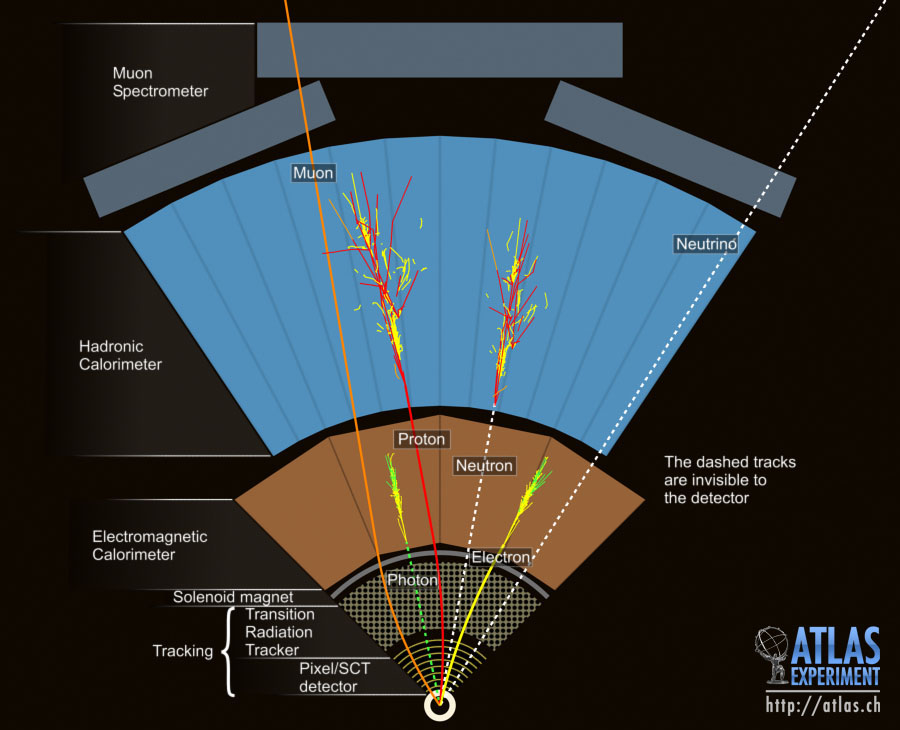
\includegraphics[scale=0.30]{Chapters/Tracks.jpg}};
\end{tikzpicture}

\end{frame}



%saptamana4
\begin{frame}{}

\vspace{-2.5cm}

\textbf{\href{https://drive.google.com/drive/folders/121cdQn74gWtBP5Rth16oqT7wxffUJkgJ}{ IV) A patra săptămână (click):}}\\
\small
\makebox[0.5cm]{}a) Corelare elementelor reale(ATLAS) cu părțile softului HYPATIA - logica detectorilor și detectarea unor semnalele utile.\\
\makebox[0.5cm]{}b) Analiza câtorva sute de evenimente și reprezentarea unor distribuții invariante de masă - evidențierea rezonanțelor aferente unor particule precum mesonii: J/\psi(~3 GeV/c2), \Upsilon(~10 Gev/c2) și bosonii de etalonare:  Z(~90 GeV/c2) + Z'(~1000 GeV/c2)(?)  \\
\makebox[0.5cm]{}c) Crearea primei prezentări LaTeX și îmbinarea unor aspecte relevante în formarea unei imagini diferite asupra naturii experimentale.\\

%Ubuntu
\begin{tikzpicture}[overlay, remember picture]
\node[anchor=center, 
      xshift=-3.5cm, 
      yshift=-1.5cm] 
     at (current page.center) 
     {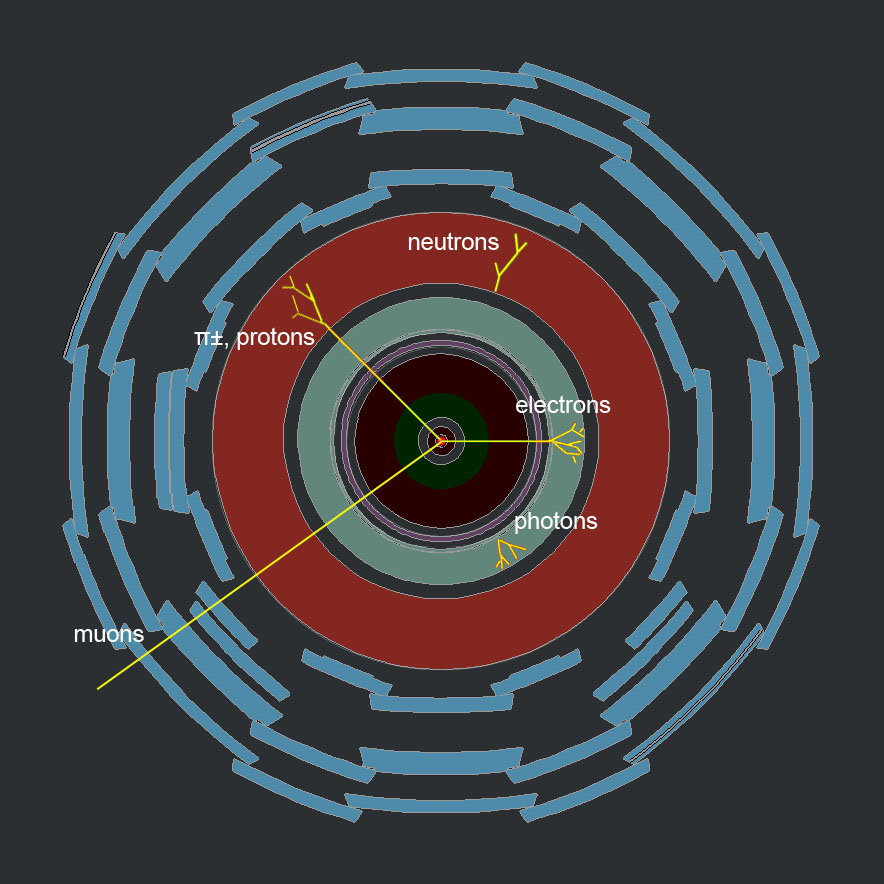
\includegraphics[scale=0.13]{Chapters/HypatCanvas.jpg}};
\end{tikzpicture}

%Ubuntu
\begin{tikzpicture}[overlay, remember picture]
\node[anchor=center, 
      xshift=2.5cm, 
      yshift=-1.5cm] 
     at (current page.center) 
     {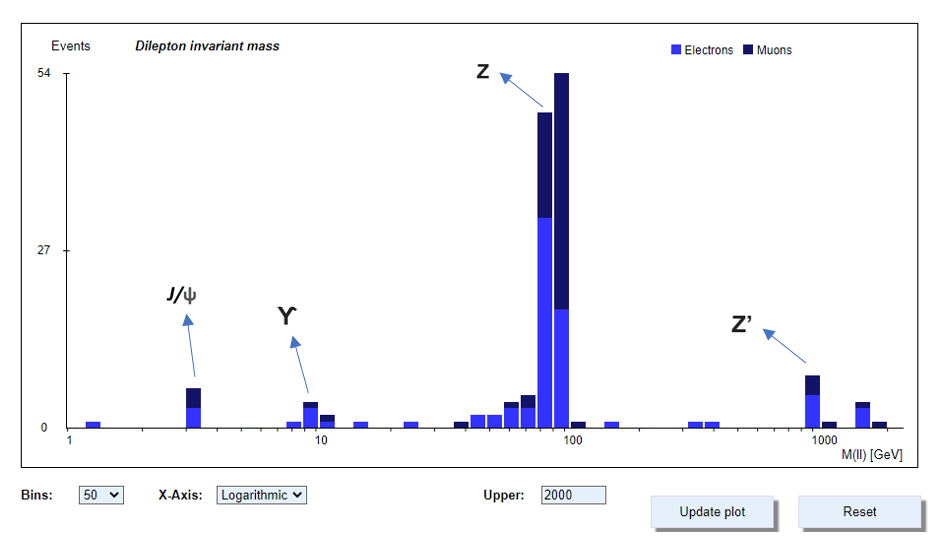
\includegraphics[scale=0.3]{Chapters/Plots.png}};
\end{tikzpicture}

\end{frame}


%histo
\begin{frame}{\textbf{Detectarea Bosonului Higgs!}}
    
\begin{tikzpicture}[overlay, remember picture]
\node[anchor=center, 
      xshift=0cm, 
      yshift=0cm] 
     at (current page.center) 
     {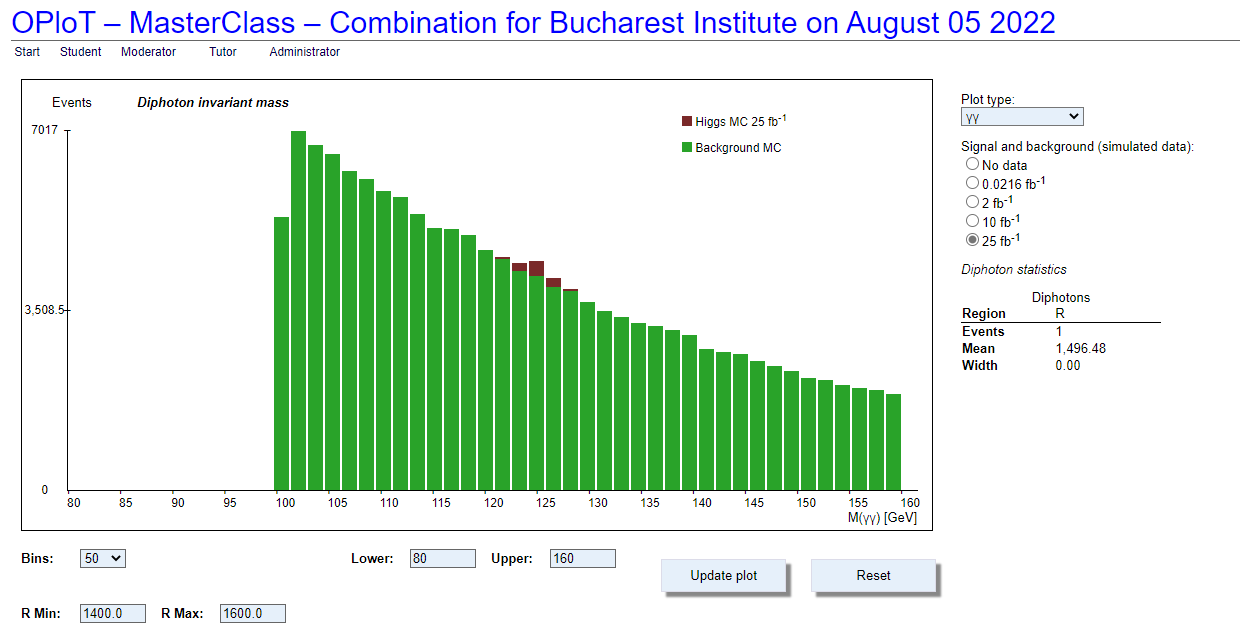
\includegraphics[scale=0.35]{Chapters/ExpectedProbability_Higgs.png}};
\end{tikzpicture}

\end{frame}

%histo
\begin{frame}{\textbf{Canale de dezintegrare}}
    
\begin{tikzpicture}[overlay, remember picture]
\node[anchor=center, 
      xshift=0cm, 
      yshift=0cm] 
     at (current page.center) 
     {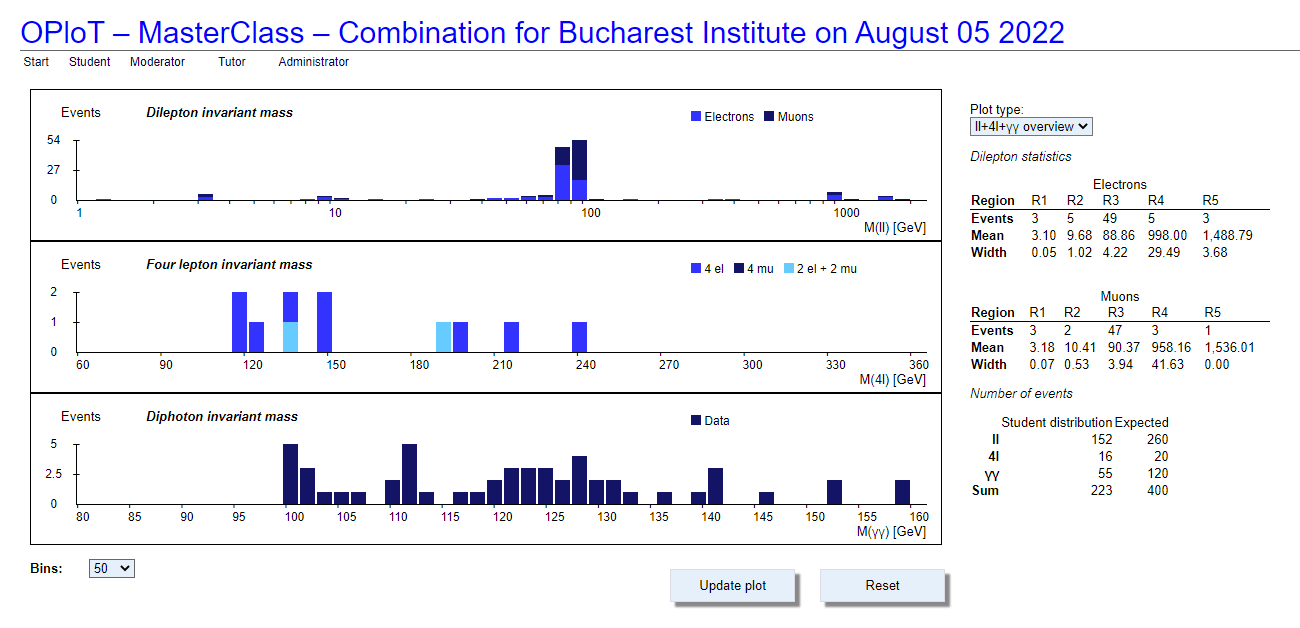
\includegraphics[scale=0.35]{Chapters/DiLeptHisto.png}};
\end{tikzpicture}

\end{frame}

%a cincea saptamana

%saptamana4
\begin{frame}{}

\vspace{-2.5cm}

 \textbf{\href{https://drive.google.com/drive/folders/1FXUY6QL6ON_hOmm1B-tGX1i_wcVkclVY}{ V) A cincea săptămână (click):}}\\

\makebox[0.5cm]{}a) Instalarea și acomodarea cu toolkit-ul GEANT4 - reactualizarea elementelor de C++(OOP).\\
\makebox[0.5cm]{}b) Descrierea elementelor unei simulări - o prezentare introductivă în GEANT4. \\
\makebox[0.5cm]{}c) Crearea unui template general și înțelegerea logicii programelor.\\
\makebox[0.5cm]{}d) Structurarea și cuantificarea cunoștințelor acumulate.\\

%Ubuntu
\begin{tikzpicture}[overlay, remember picture]
\node[anchor=center, 
      xshift=-3.5cm, 
      yshift=-1cm] 
     at (current page.center) 
     {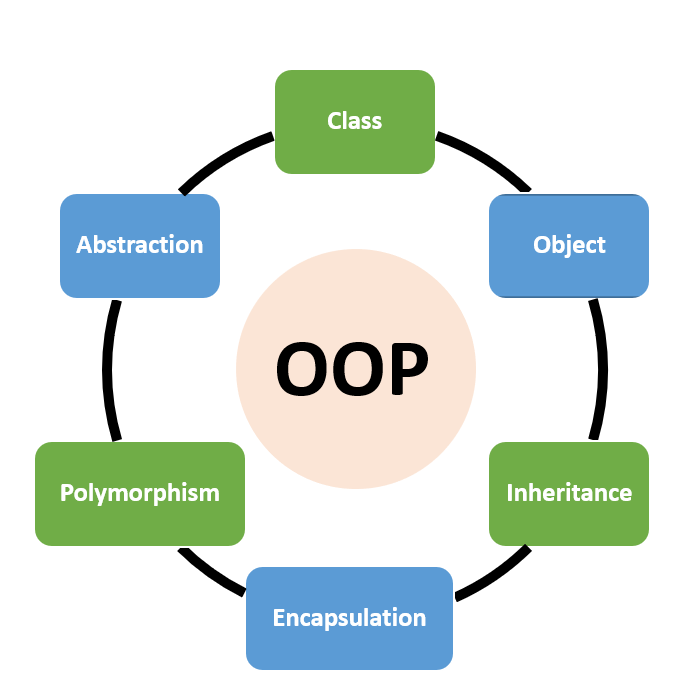
\includegraphics[scale=0.26]{Chapters/OOP_class3.png}};
\end{tikzpicture}

%Ubuntu
\begin{tikzpicture}[overlay, remember picture]
\node[anchor=center, 
      xshift=2.5cm, 
      yshift=-1.5cm] 
     at (current page.center) 
     {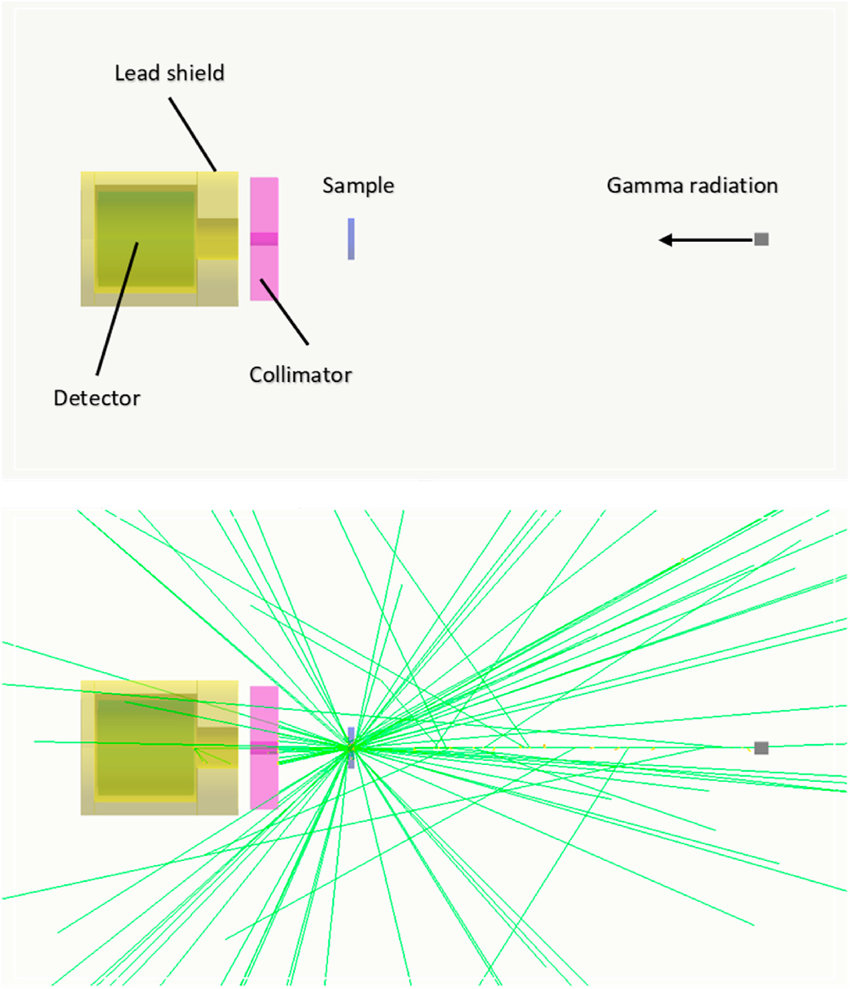
\includegraphics[scale=0.14]{Chapters/Visualization-of-the-Geant4-simulation-code.jpg}};
\end{tikzpicture}

\begin{tikzpicture}[overlay, remember picture]
\node[anchor=center, 
      xshift=-3.5cm, 
      yshift=-3.5cm] 
     at (current page.center) 
     {
\includegraphics[scale=0.2]{Chapters/g4logo-full.png}};
\end{tikzpicture}

\end{frame}


\begin{frame}{\textbf{Clasele de bază - structura unui program}}
    
\begin{tikzpicture}[overlay, remember picture]
\node[anchor=center, 
      xshift=0cm, 
      yshift=-0.5cm] 
     at (current page.center) 
     {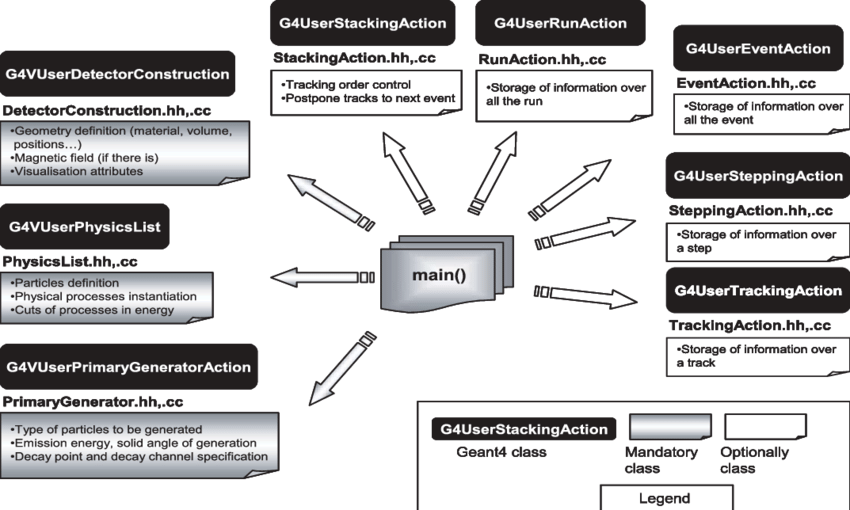
\includegraphics[scale=0.35]{Chapters/Mandatory-and-some-optionally-classes-needed-by-a-GEANT4-based-application.png}};
\end{tikzpicture}

\end{frame}

%sapt6- Detectorul de radiatie Cherenkov
\begin{frame}{}

\vspace{-2.5cm}

 \textbf{\href{https://drive.google.com/drive/folders/1zzlqdGbWhLVaXbJWPfIV9lElrCDSFFmS}{ VI) A șasea săptămână (click)}}\\

\makebox[0.5cm]{}a) Crearea primei simulări grafice în G4 - detectorul de radiație Cherenkov.\\
\makebox[0.5cm]{}b) Ajustarea și corelarea structurilor de cod necesare rulării programului. \\
\makebox[0.5cm]{}c) Depanarea codului - corectarea erorilor(Debugging).\\
\makebox[0.5cm]{}d) Punerea în practică a bazelor cunoștințelor acumulate.\\

%Ubuntu
\begin{tikzpicture}[overlay, remember picture]
\node[anchor=center, 
      xshift=-3.5cm, 
      yshift=0cm] 
     at (current page.center) 
     {
\includegraphics[scale=0.3]{Chapters/g4logo-full.png }};
\end{tikzpicture}

%Ubuntu
\begin{tikzpicture}[overlay, remember picture]
\node[anchor=center, 
      xshift=2.5cm, 
      yshift=-1.5cm] 
     at (current page.center) 
     {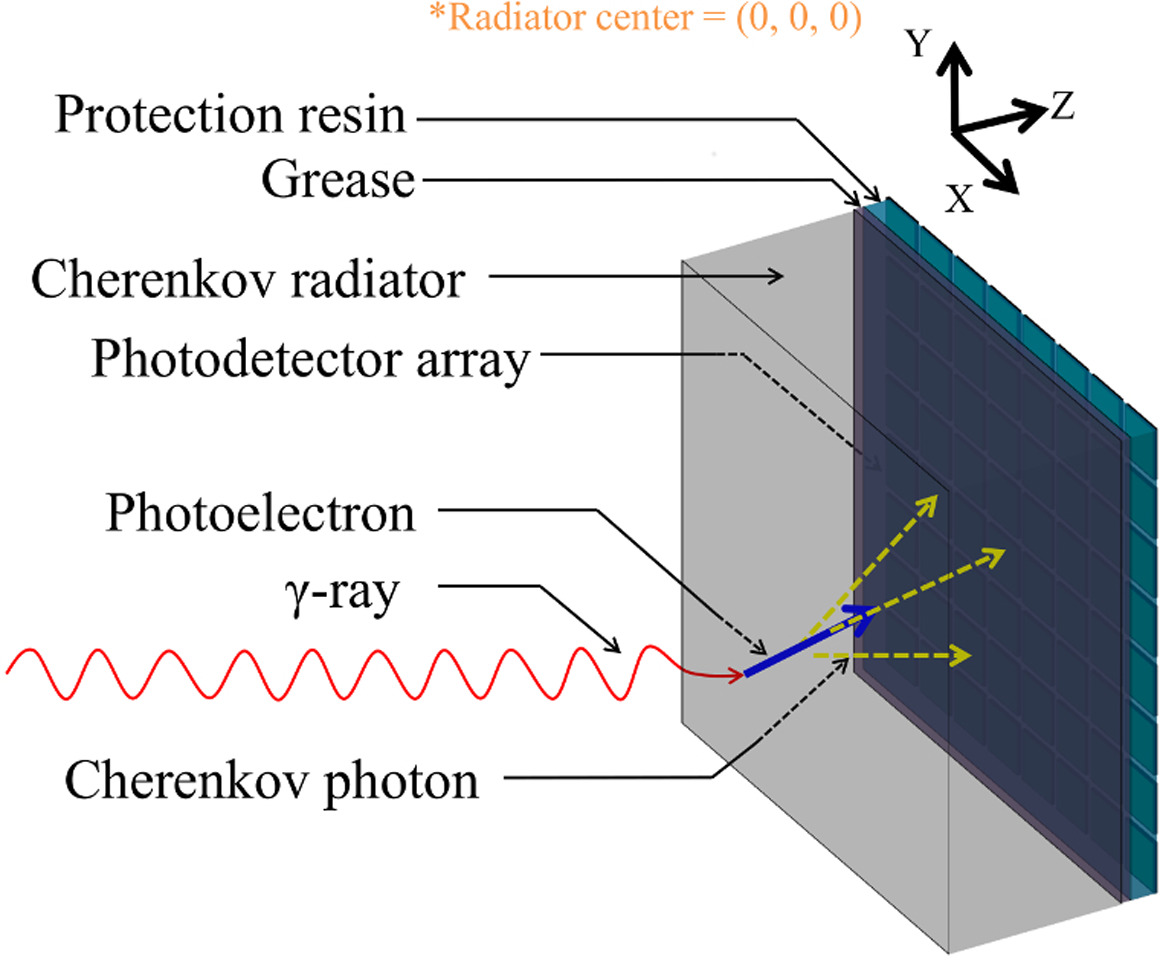
\includegraphics[scale=0.8]{Chapters/mp12851-fig-0001-m.jpg}};
\end{tikzpicture}

\begin{tikzpicture}[overlay, remember picture]
\node[anchor=center, 
      xshift=-3.5cm, 
      yshift=-2cm] 
     at (current page.center) 
     {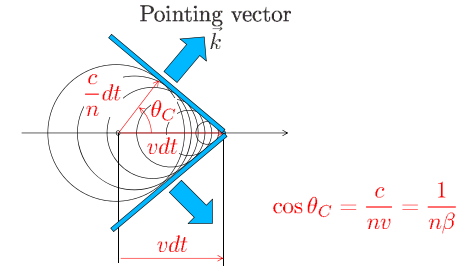
\includegraphics[scale=0.34]{Chapters/cerk.png}};
\end{tikzpicture}

\end{frame}

%100 events

\begin{frame}
    
\begin{tikzpicture}[overlay, remember picture]
\node[anchor=center, 
      xshift=0cm, 
      yshift=0cm] 
     at (current page.center) 
     {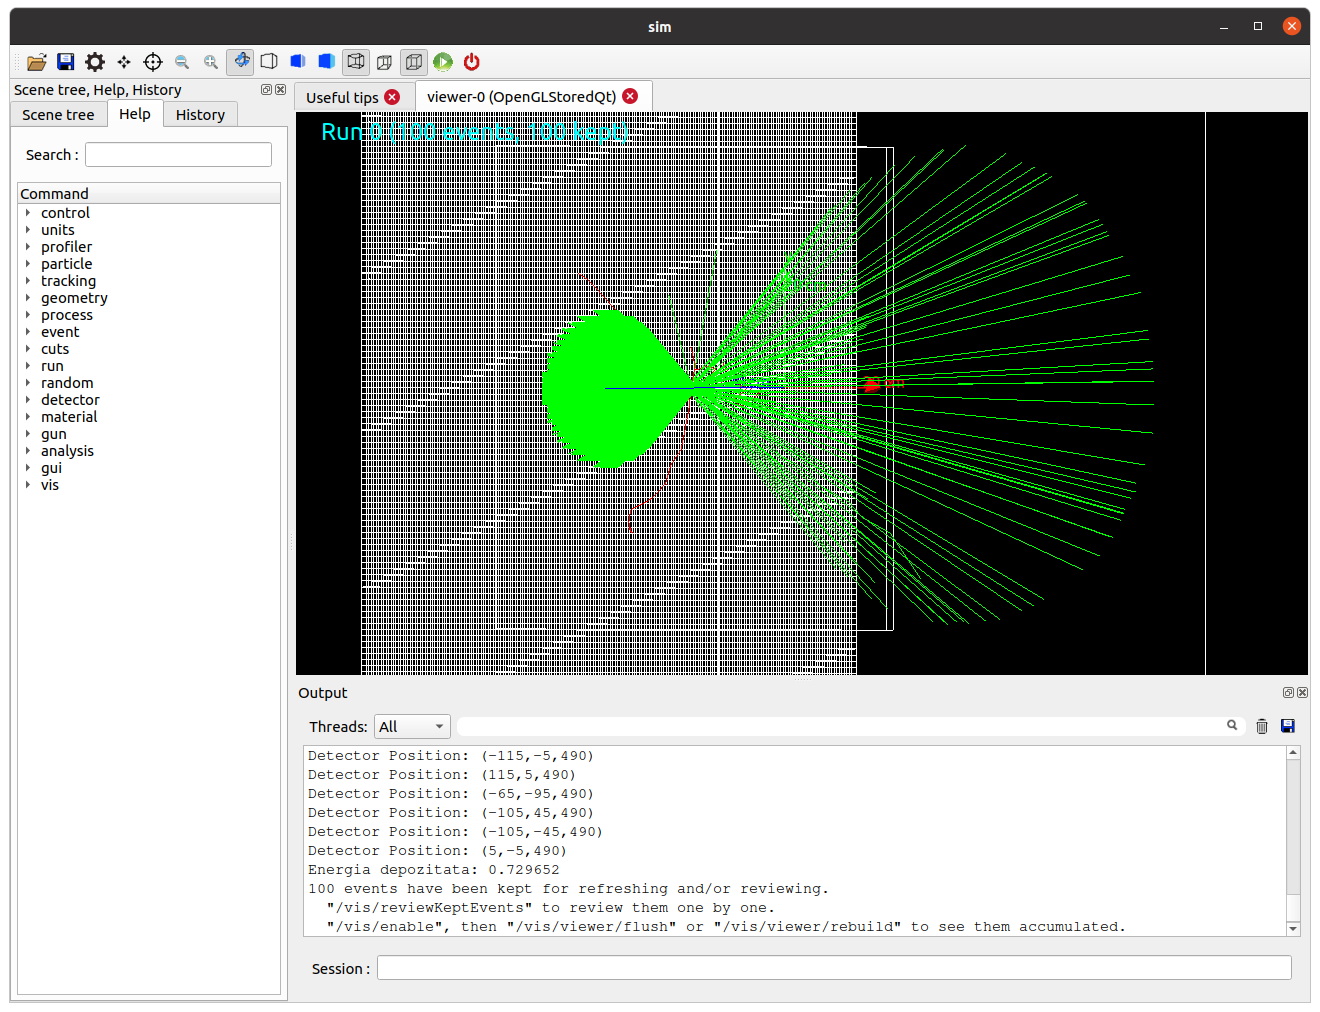
\includegraphics[scale=0.3]{Chapters/100 Events.png}};
\end{tikzpicture}

\end{frame}

\begin{frame}
    
\begin{tikzpicture}[overlay, remember picture]
\node[anchor=center, 
      xshift=0cm, 
      yshift=0cm] 
     at (current page.center) 
     {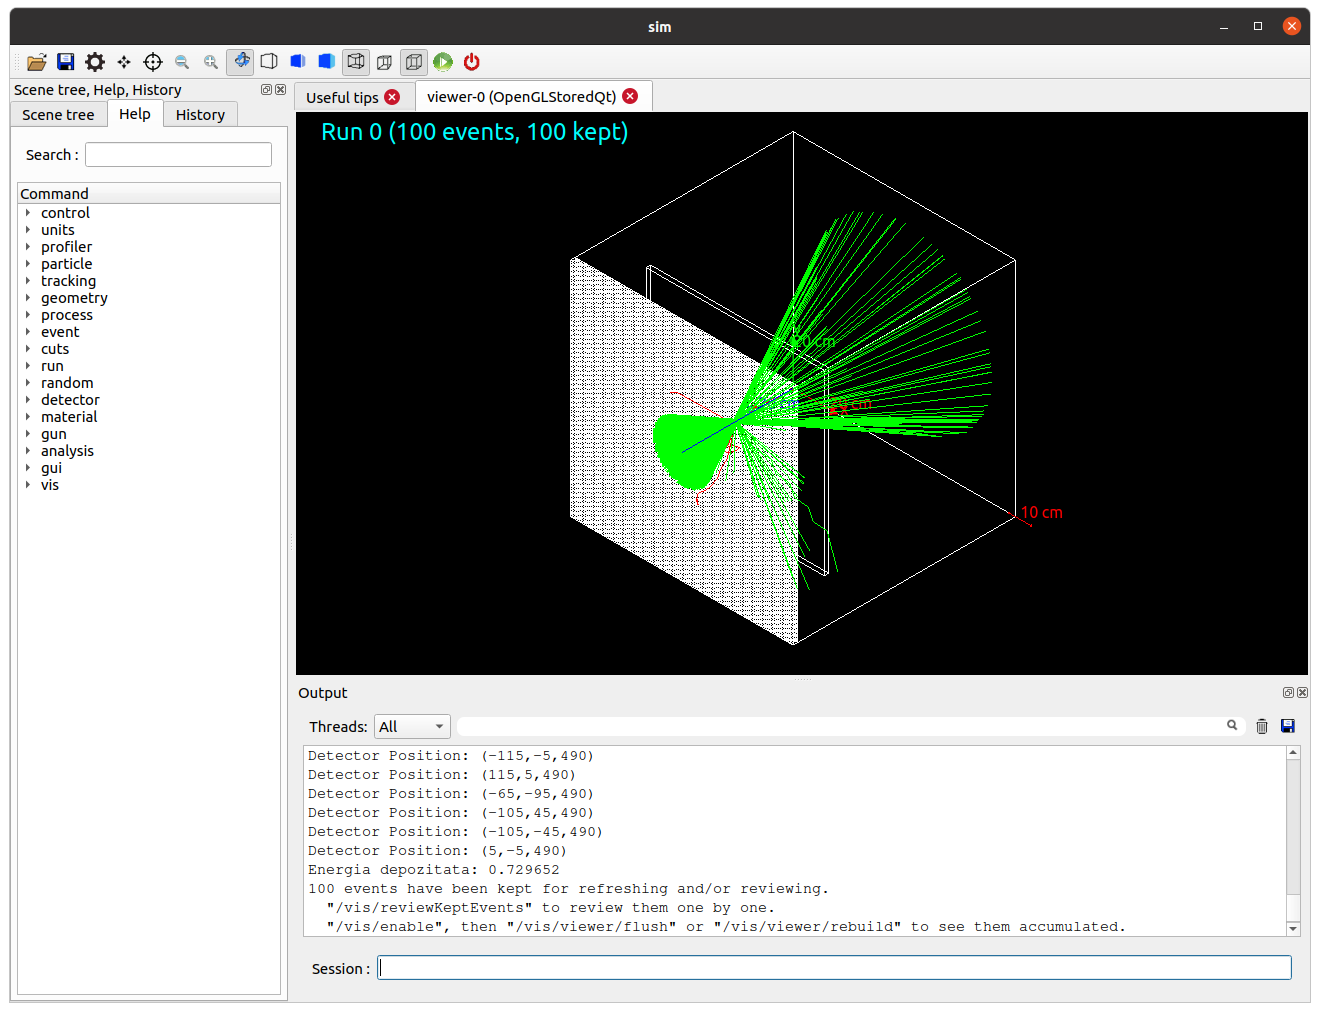
\includegraphics[scale=0.22]{Chapters/GUI- gemoetry.png}};
\end{tikzpicture}

\end{frame}


\begin{frame}{\textbf{Distribuție nr. Fotoni/Eveniment}}
    
\begin{tikzpicture}[overlay, remember picture]
\node[anchor=center, 
      xshift=0cm, 
      yshift=0cm] 
     at (current page.center) 
     {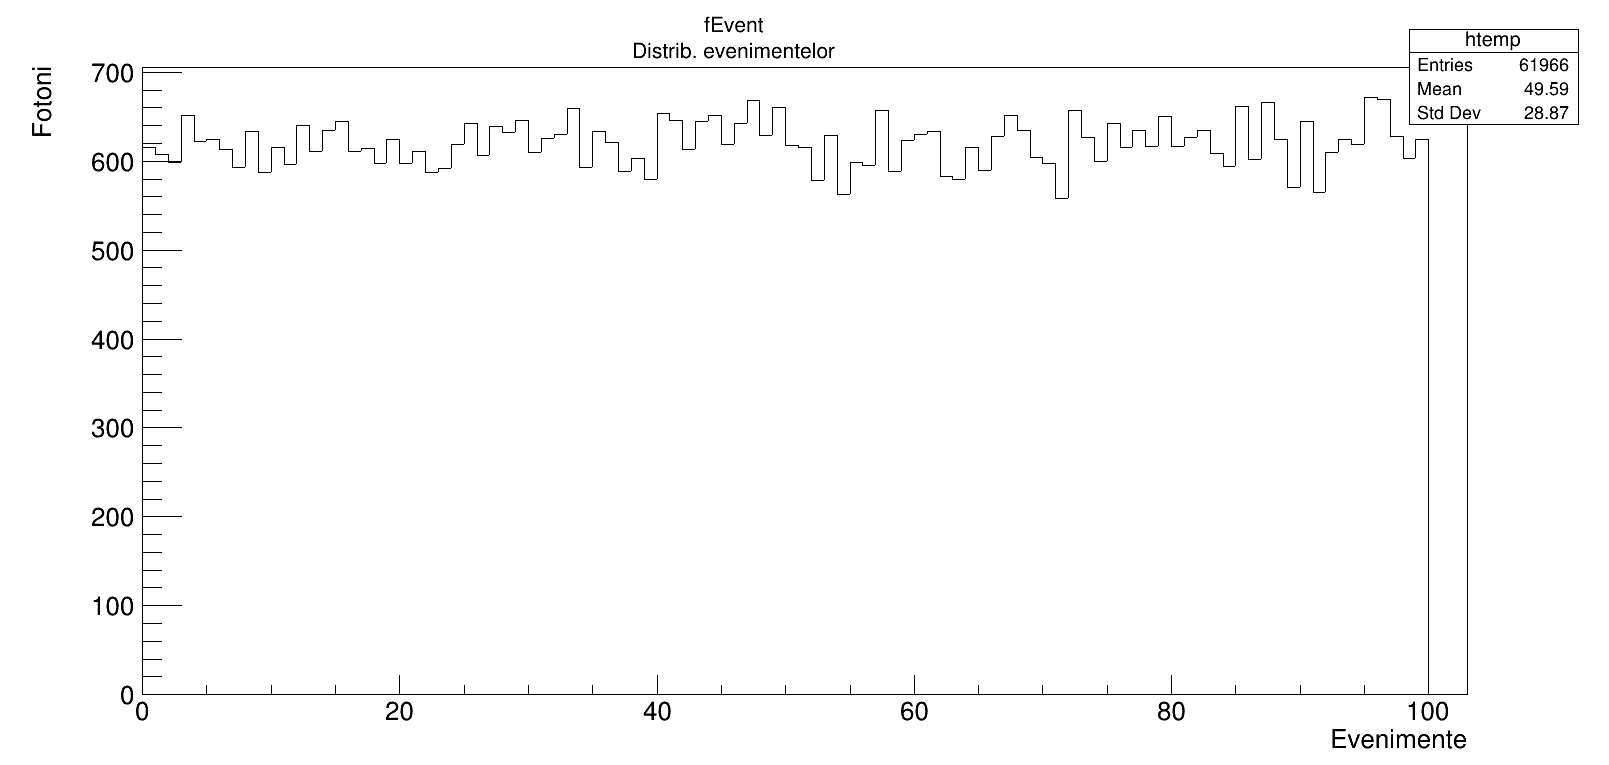
\includegraphics[scale=0.22]{Chapters/Distribuție1.png}};
\end{tikzpicture}

\end{frame}


%Hits Distribution

\begin{frame}{\textbf{Distribuție de senzori - OX}}
    
\begin{tikzpicture}[overlay, remember picture]
\node[anchor=center, 
      xshift=0cm, 
      yshift=0cm] 
     at (current page.center) 
     {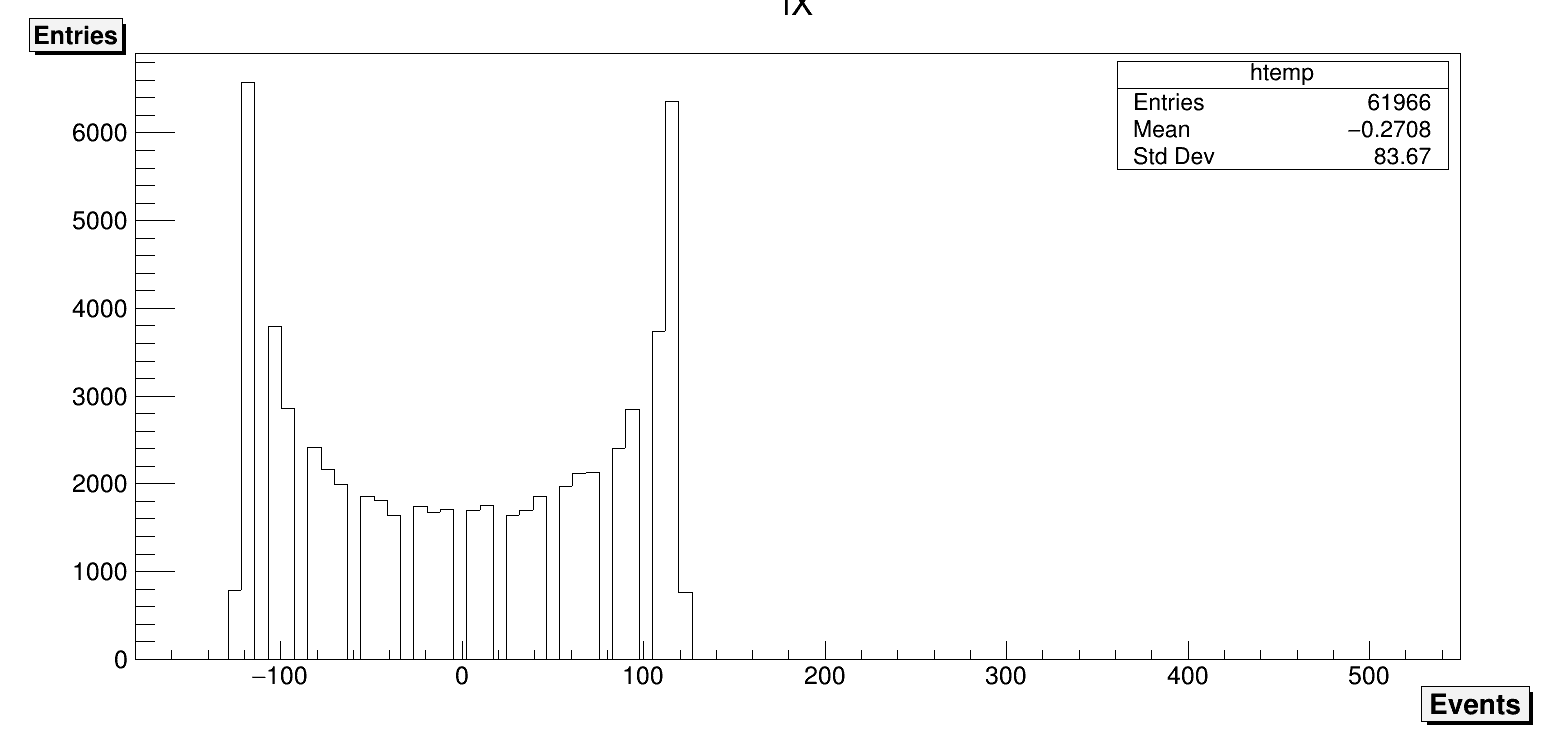
\includegraphics[scale=0.25]{Chapters/Ox-hits distribution.png}};
\end{tikzpicture}

\end{frame}



\begin{frame}{\textbf{Distribuție de senzori - OY}}
    
\begin{tikzpicture}[overlay, remember picture]
\node[anchor=center, 
      xshift=0cm, 
      yshift=0cm] 
     at (current page.center) 
     {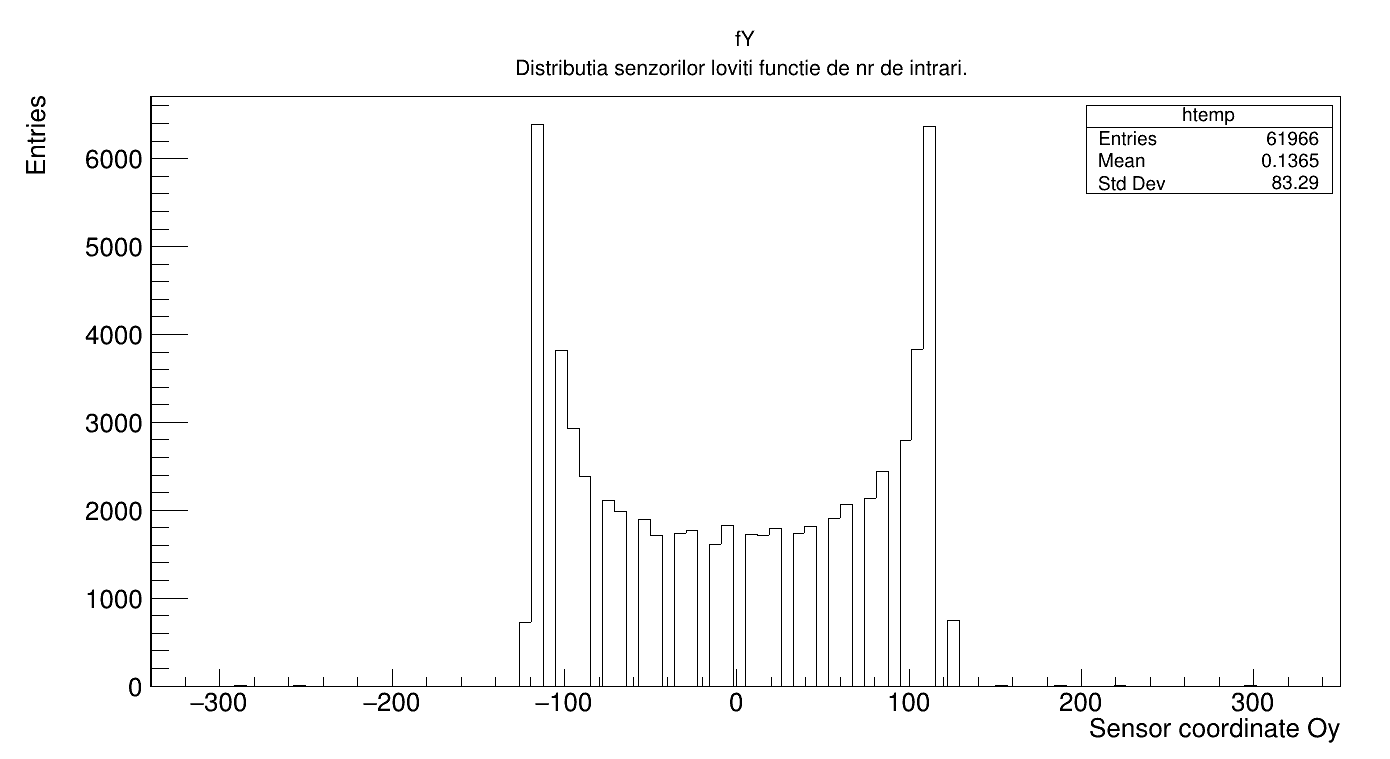
\includegraphics[scale=0.25]{Chapters/Oy-hits distribution.png}};
\end{tikzpicture}

\end{frame}


\begin{frame}{\textbf{Spectrul radiației Cherenkov}}
    
\begin{tikzpicture}[overlay, remember picture]
\node[anchor=center, 
      xshift=0cm, 
      yshift=0cm] 
     at (current page.center) 
     {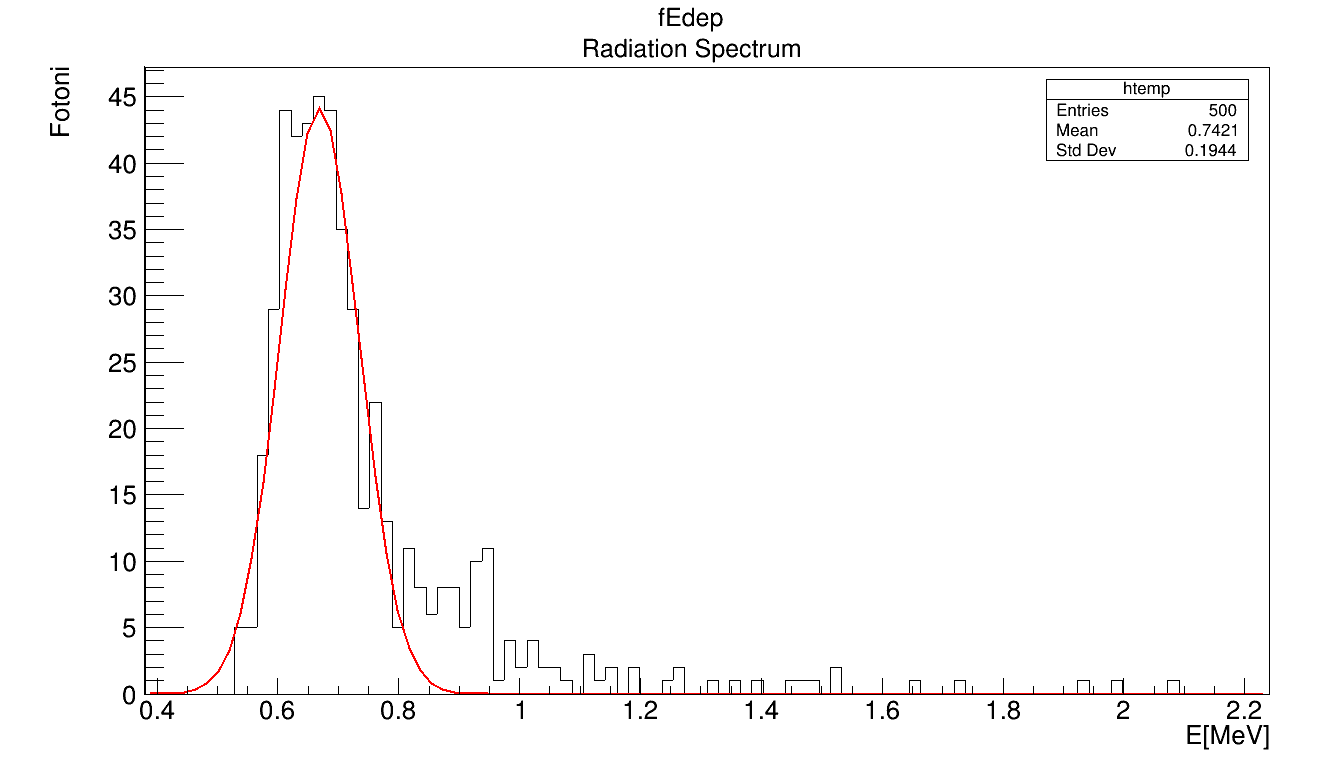
\includegraphics[scale=0.25]{Chapters/Radiation SPectrum.png}};
\end{tikzpicture}

\end{frame}


%Ring plot
\begin{frame}{\textbf{Ring Pattern - Corelarea Datelor}}
    
\begin{tikzpicture}[overlay, remember picture]
\node[anchor=center, 
      xshift=0cm, 
      yshift=0cm] 
     at (current page.center) 
     {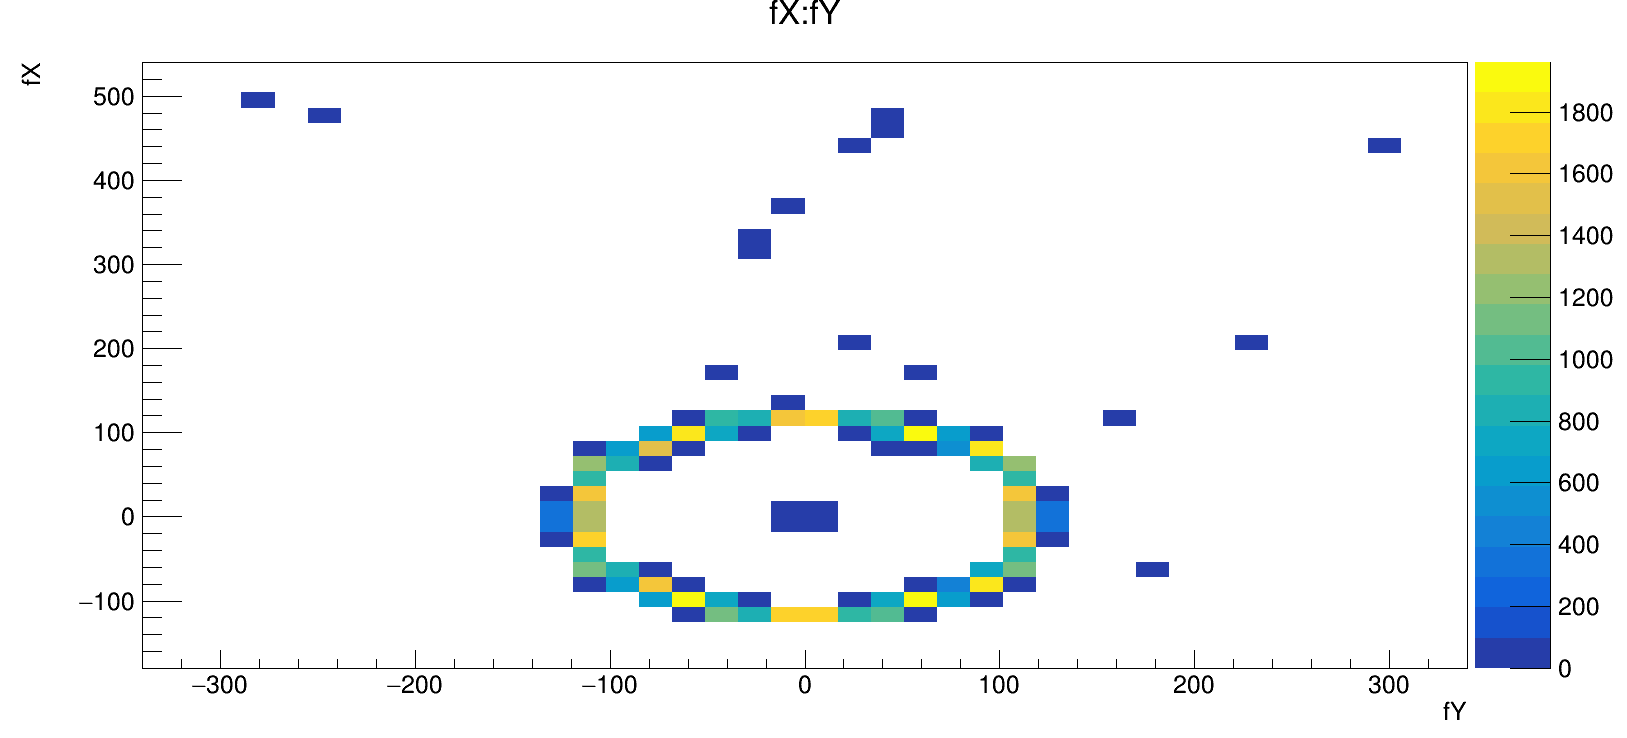
\includegraphics[scale=0.24]{Chapters/Ring Corelation Ox-Oy.png}};
\end{tikzpicture}

\end{frame}


%real ring
\begin{frame}{\textbf{Ring Pattern - output grafic}}
    
\begin{tikzpicture}[overlay, remember picture]
\node[anchor=center, 
      xshift=0cm, 
      yshift=0cm] 
     at (current page.center) 
     {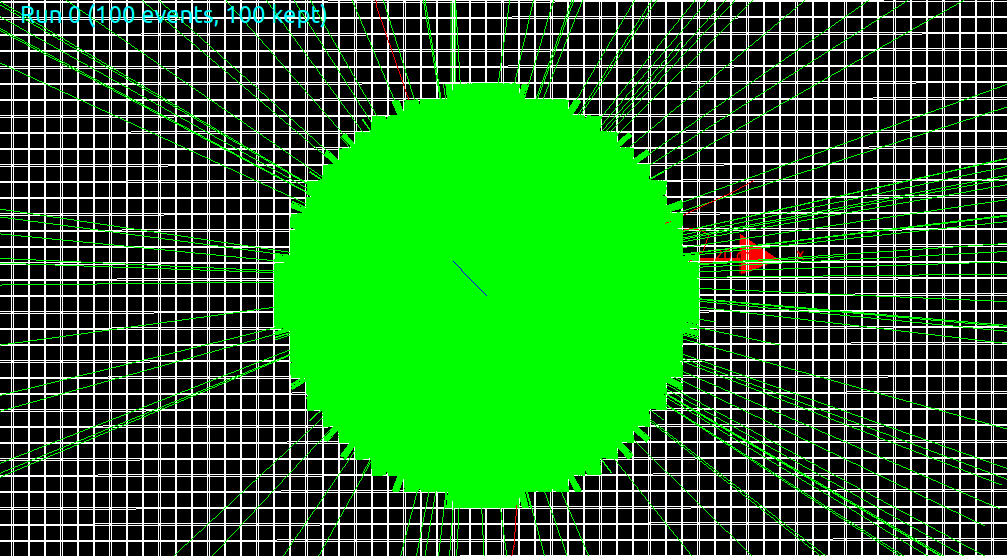
\includegraphics[scale=0.3]{Chapters/RealRing.png}};
\end{tikzpicture}

\end{frame}

%QE
\begin{frame}{\textbf{Eficiența cuantică}}
    
\begin{tikzpicture}[overlay, remember picture]
\node[anchor=center, 
      xshift=0cm, 
      yshift=0cm] 
     at (current page.center) 
     {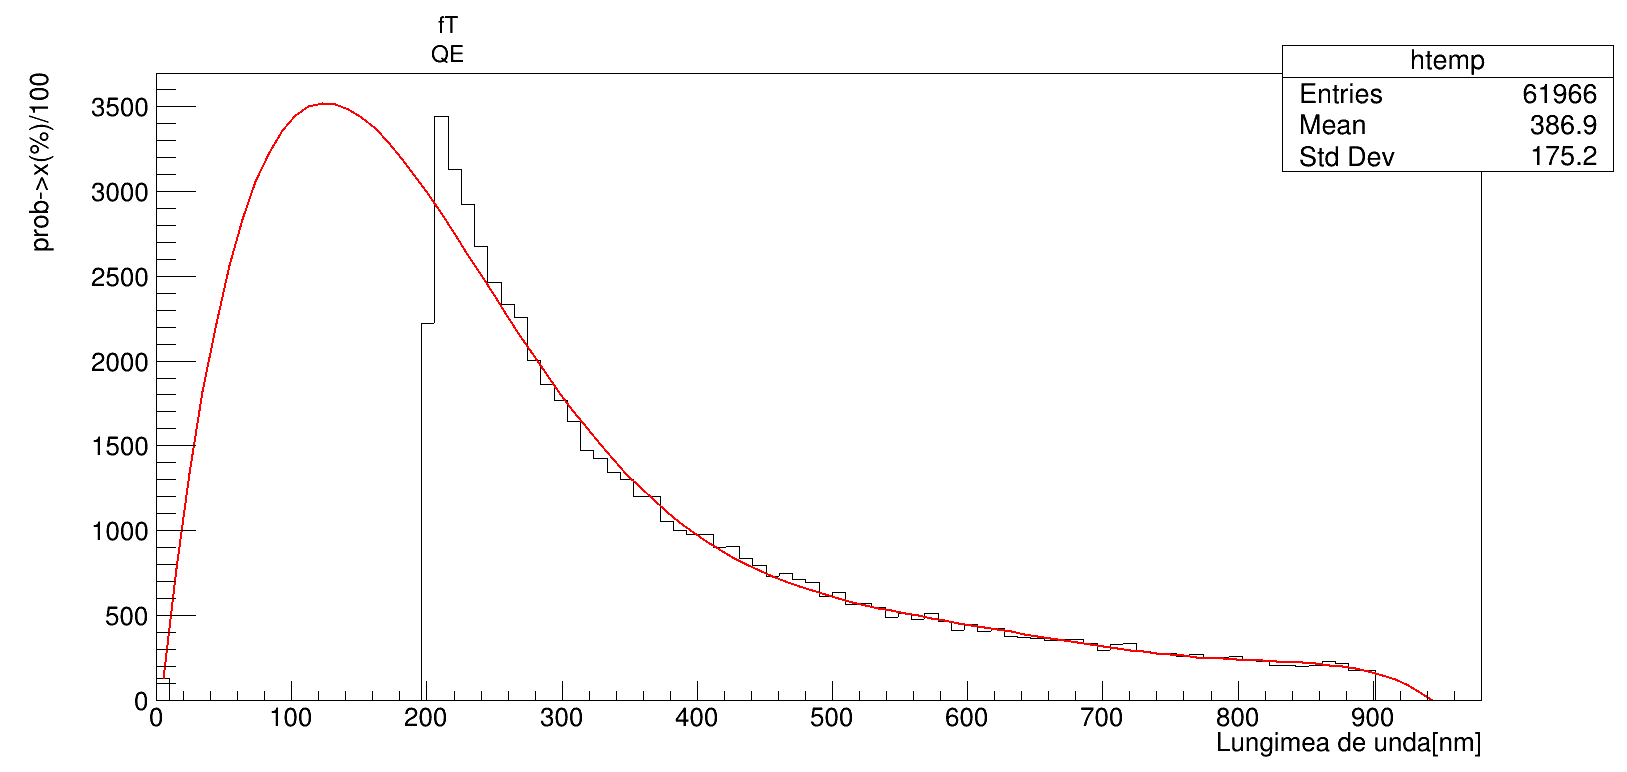
\includegraphics[scale=0.22]{Chapters/Eficienta Cuantica.png}};
\end{tikzpicture}

\end{frame}


\begin{frame}{}

\vspace{-2.5cm}

\textbf{\href{https://drive.google.com/drive/folders/1U9p1sCGWZ7dWKFcxKtc8qLJI4uPMXXod}{VII) Săptămânile 7 și 8 (click):}}\\

\makebox[0.5cm]{}a) Simularea unui detector cu Ge hiperpur.\\
\makebox[0.5cm]{}b) Plotarea câtorva spectre de distribuție. \\
\makebox[0.5cm]{}c) Depanarea codului - corectarea erorilor(Debugging).\\
\makebox[0.5cm]{}d) Definirea unor aspecte particulare.\\


\begin{tikzpicture}[overlay, remember picture]
\node[anchor=center, 
      xshift=-3.5cm, 
      yshift=0cm] 
     at (current page.center) 
     {
\includegraphics[scale=0.3]{Chapters/g4logo-full.png }};
\end{tikzpicture}


\begin{tikzpicture}[overlay, remember picture]
\node[anchor=center, 
      xshift=2.5cm, 
      yshift=-1.5cm] 
     at (current page.center) 
     {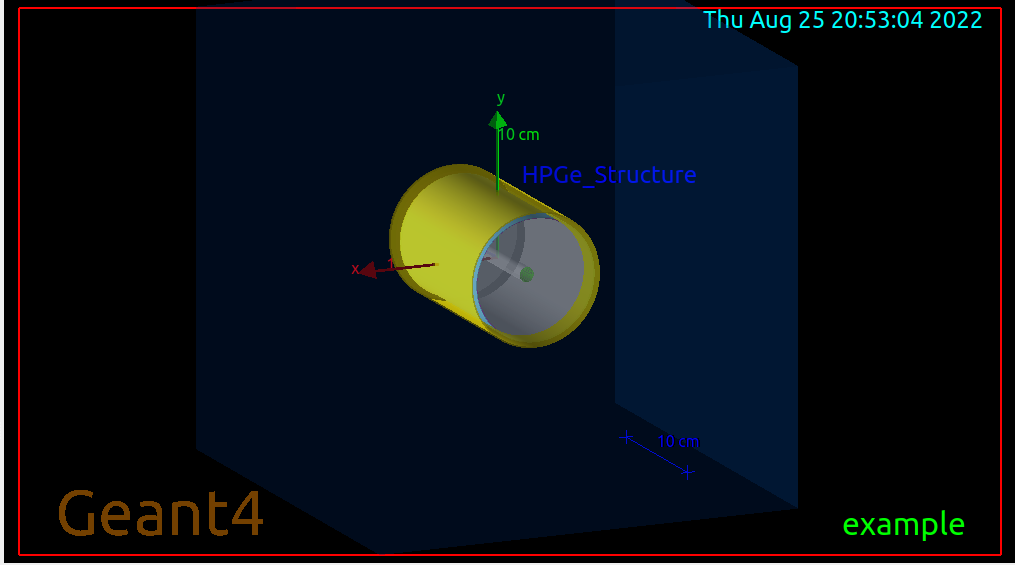
\includegraphics[scale=0.2]{Chapters/HGPE_Detector_Geometry.png}};
\end{tikzpicture}

\begin{tikzpicture}[overlay, remember picture]
\node[anchor=center, 
      xshift=-3.5cm, 
      yshift=-2.5cm] 
     at (current page.center) 
     {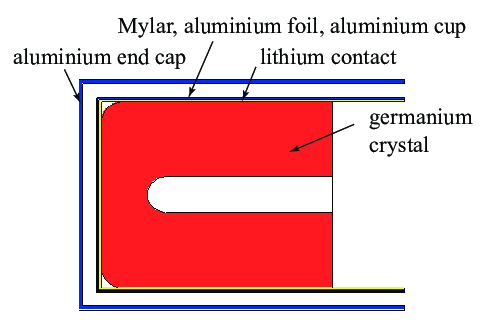
\includegraphics[scale=0.2]{Chapters/Schematic-representation-of-HPGe-detector-Aluminium-is-represented-in-dark-blue-and.png}};
\end{tikzpicture}

\end{frame}

\begin{frame}{\textbf{HPGe detector parts}}
    
\begin{tikzpicture}[overlay, remember picture]
\node[anchor=center, 
      xshift=-3cm, 
      yshift=1cm] 
     at (current page.center) 
     {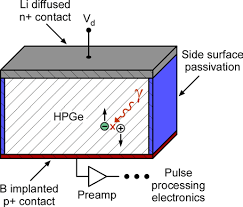
\includegraphics[scale=0.45]{Chapters/GammaDetector.png}};
\end{tikzpicture}

\begin{tikzpicture}[overlay, remember picture]
\node[anchor=center, 
      xshift=3cm, 
      yshift=-1cm] 
     at (current page.center) 
     {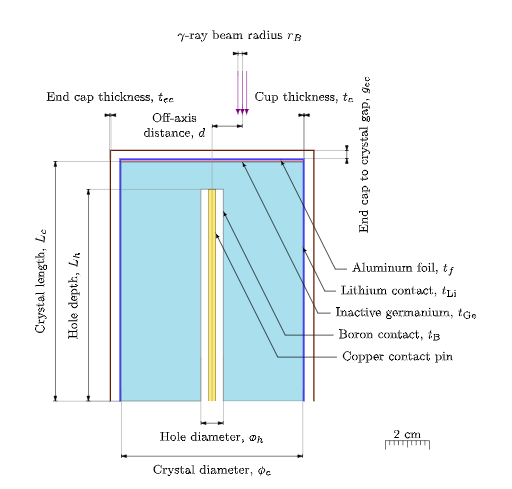
\includegraphics[scale=0.45]{Chapters/Ex.png}};
\end{tikzpicture}

   
\begin{tikzpicture}[overlay, remember picture]
\node[anchor=center, 
      xshift=-3.2cm, 
      yshift=-2.5cm] 
     at (current page.center) 
     {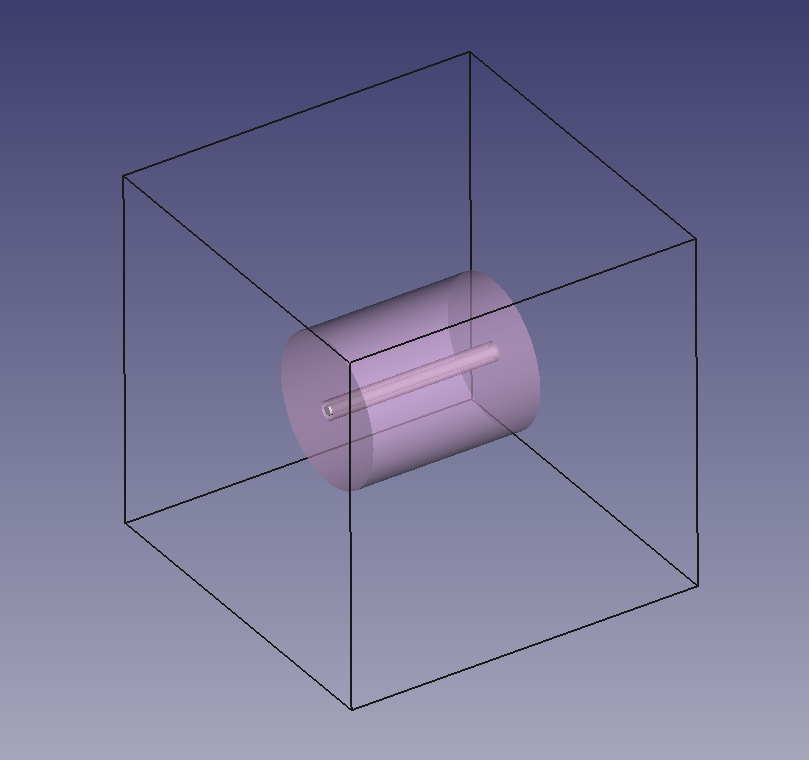
\includegraphics[scale=0.15]{Chapters/FreecadDesign.png}};
\end{tikzpicture}

\end{frame}




%Geometry
\begin{frame}{\textbf{Spectrul simulat al izotopului de Co-57}}
    
\begin{tikzpicture}[overlay, remember picture]
\node[anchor=center, 
      xshift=0cm, 
      yshift=0cm] 
     at (current page.center) 
     {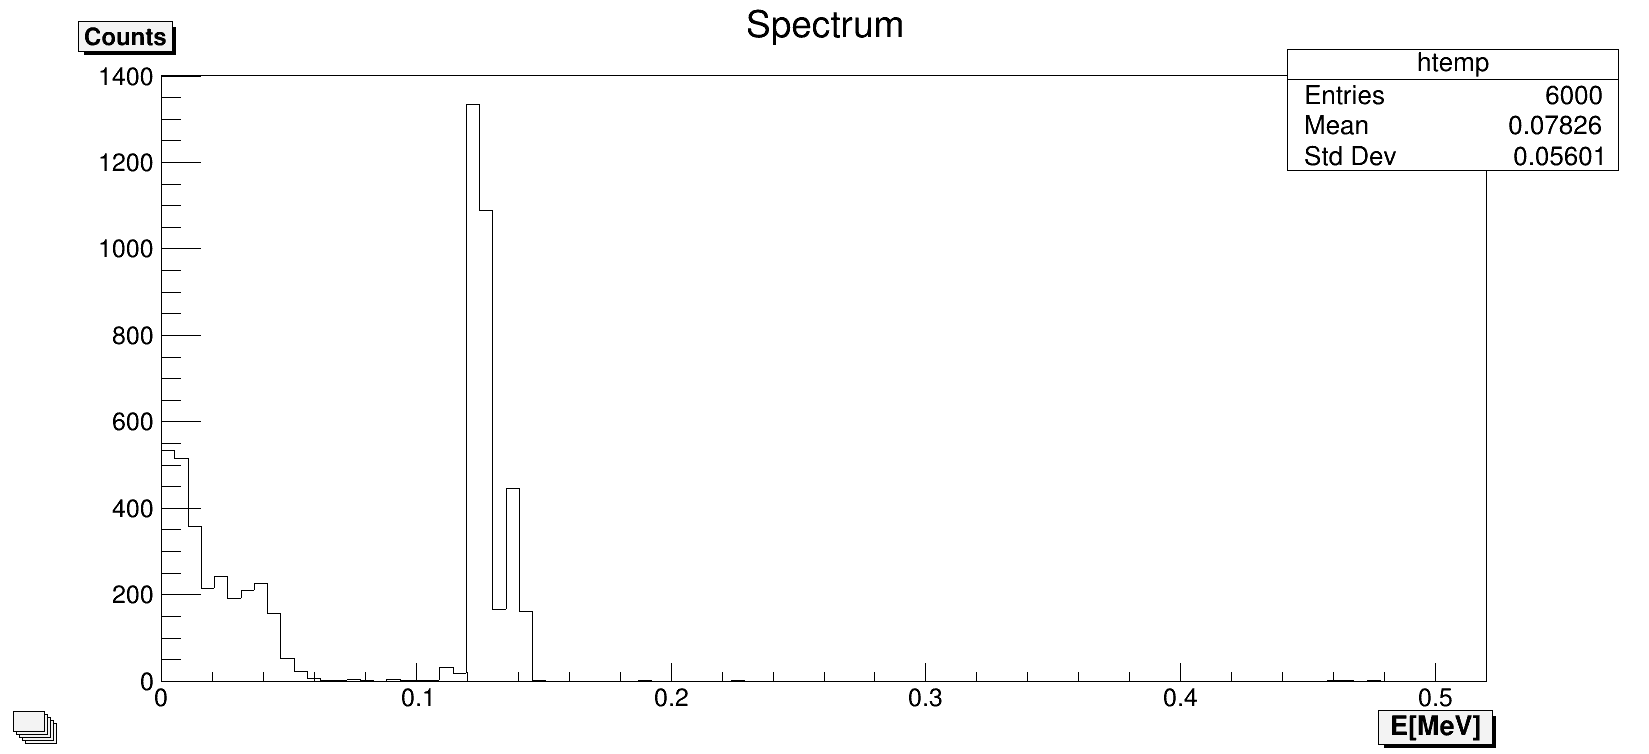
\includegraphics[scale=0.22]{Chapters/Co-57(Simulation).png}};
\end{tikzpicture}

\end{frame}


%real Eu-152
\begin{frame}{\textbf{Spectrul simulat al izotopului de Eu-152}}
    
\begin{tikzpicture}[overlay, remember picture]
\node[anchor=center, 
      xshift=0cm, 
      yshift=0cm] 
     at (current page.center) 
     {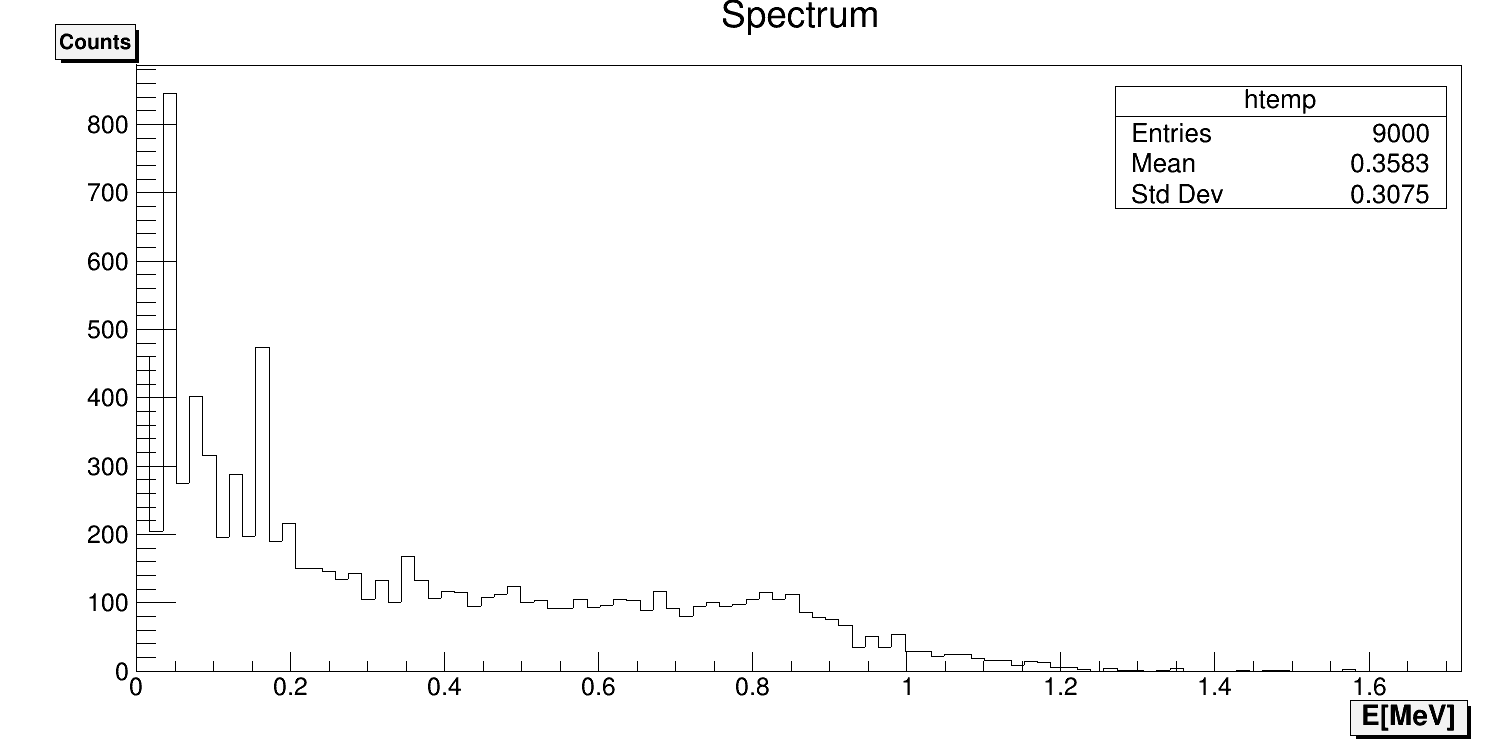
\includegraphics[scale=0.22]{Chapters/Eu-125(simulation).png}};
\end{tikzpicture}

\end{frame}


%real Eu-152
\begin{frame}{\textbf{Spectrul simulat al izotopului de Po-210}}
    
\begin{tikzpicture}[overlay, remember picture]
\node[anchor=center, 
      xshift=0cm, 
      yshift=0cm] 
     at (current page.center) 
     {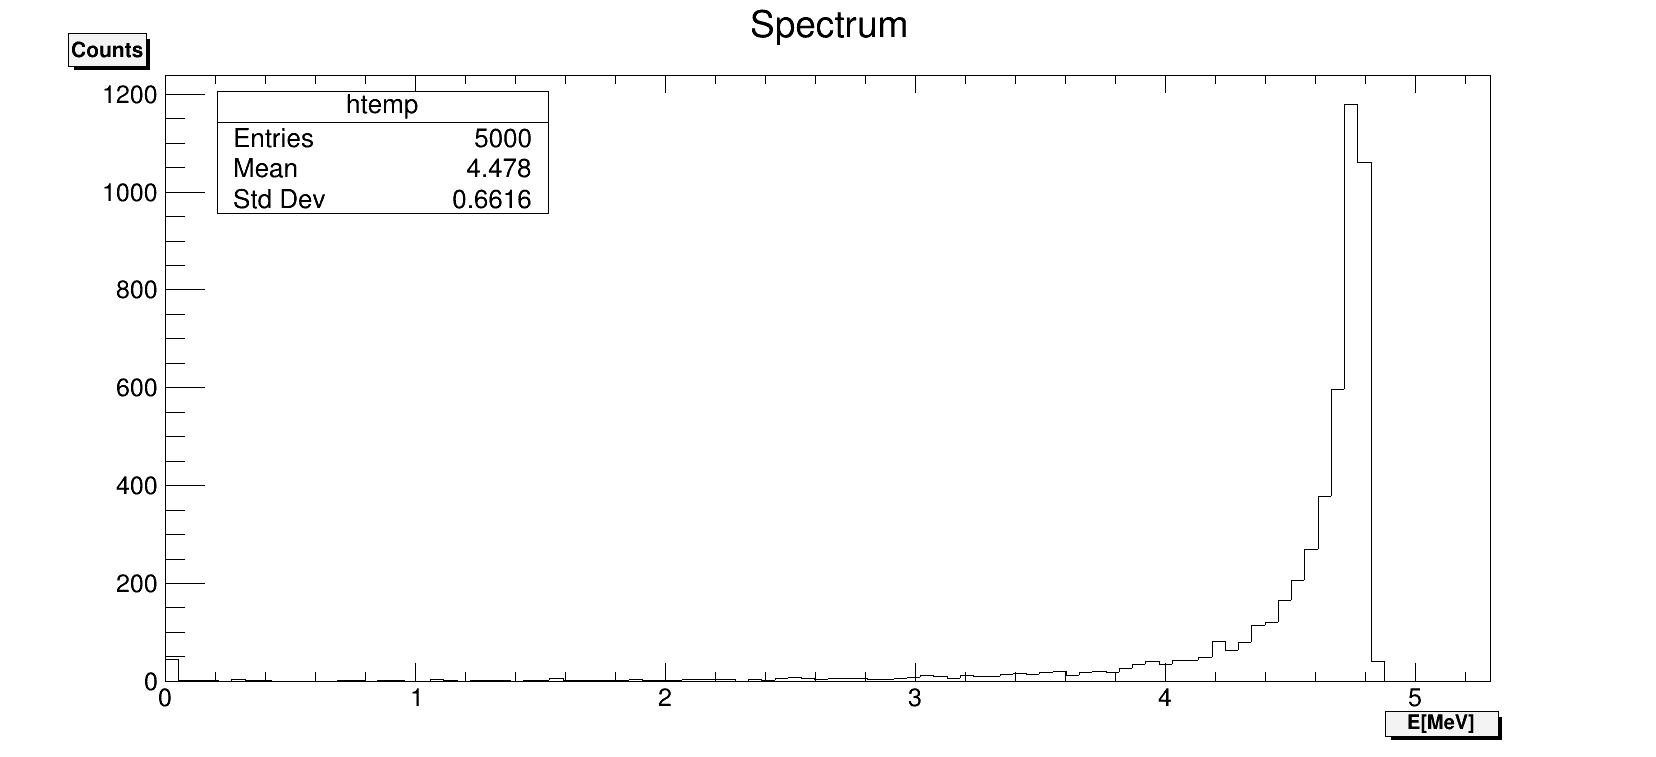
\includegraphics[scale=0.22]{Chapters/Po-210(simulation).png}};
\end{tikzpicture}

\end{frame}

%gamma source
\begin{frame}{\textbf{Spectrul simulat al unei surse gamma}}
    
\begin{tikzpicture}[overlay, remember picture]
\node[anchor=center, 
      xshift=0cm, 
      yshift=0cm] 
     at (current page.center) 
     {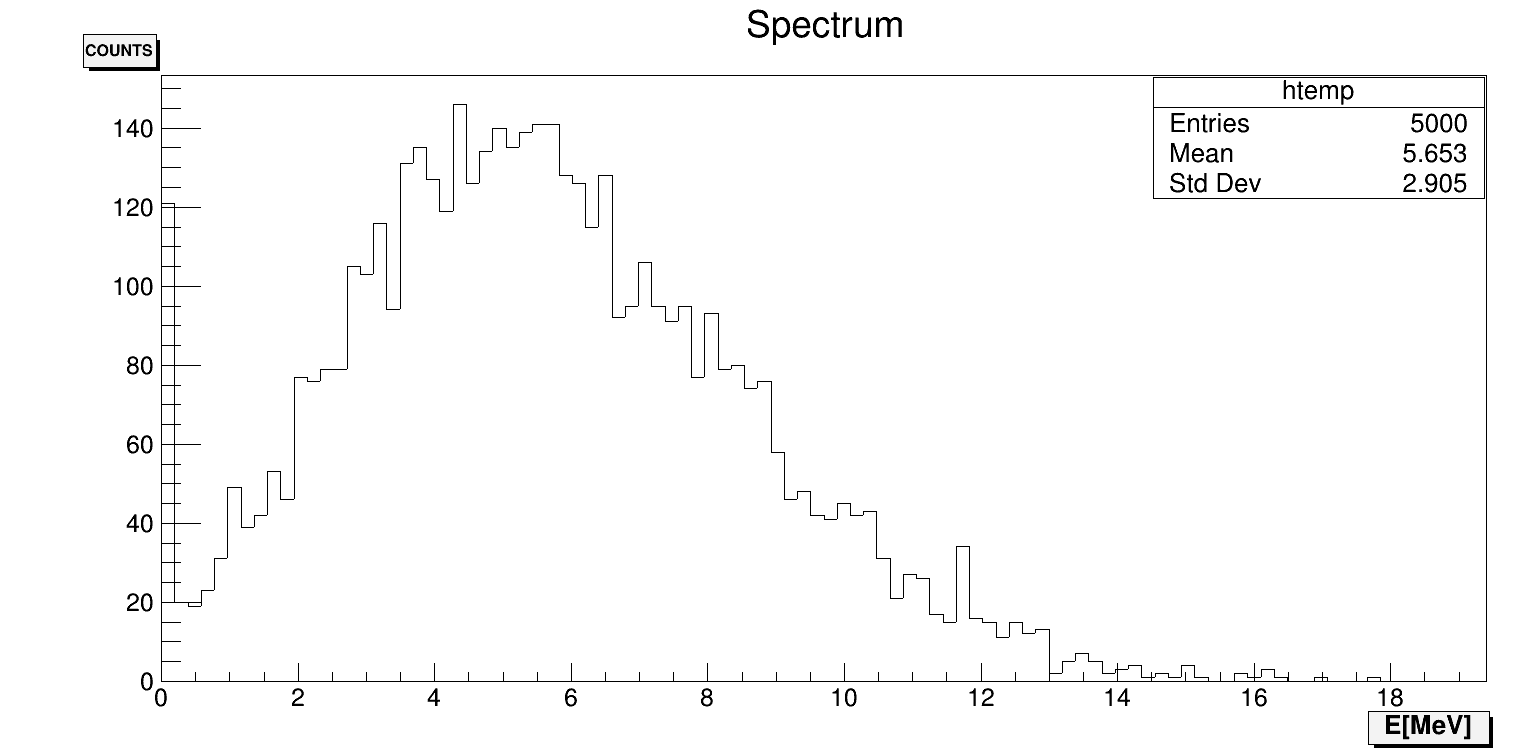
\includegraphics[scale=0.22]{Chapters/6MeV gamma.png}};
\end{tikzpicture}

\end{frame}


%jetul atmosferic
\begin{frame}

\vspace{-3cm}
\textbf{\href{https://drive.google.com/drive/folders/1R8C5VpdrXX3Mw2KU4s0h860fenNMMSye}{VIII) Săptămâna 9 (click):}}\\


\makebox[0.5cm]{}a) Simularea jetului atmosferic indus de un proton cu Ec = 100 GeV.\\
\makebox[0.5cm]{}b) Afișarea grafică a output-ului - semnăturile particulelor generate.\\
\makebox[0.5cm]{}c) Manipularea unui repository pe GitHub.\\
\makebox[0.5cm]{}d) O prezentare LaTeX despre analiza fenomenelor fizice din spatele proiectelor.\\

\begin{tikzpicture}[overlay, remember picture]
\node[anchor=center, 
      xshift=2.8cm, 
      yshift=1.5cm] 
     at (current page.center) 
     {
\includegraphics[scale=0.25]{Chapters/g4logo-full.png }};
\end{tikzpicture}


\begin{tikzpicture}[overlay, remember picture]
\node[anchor=center, 
      xshift=2.5cm, 
      yshift=-1.5cm] 
     at (current page.center) 
     {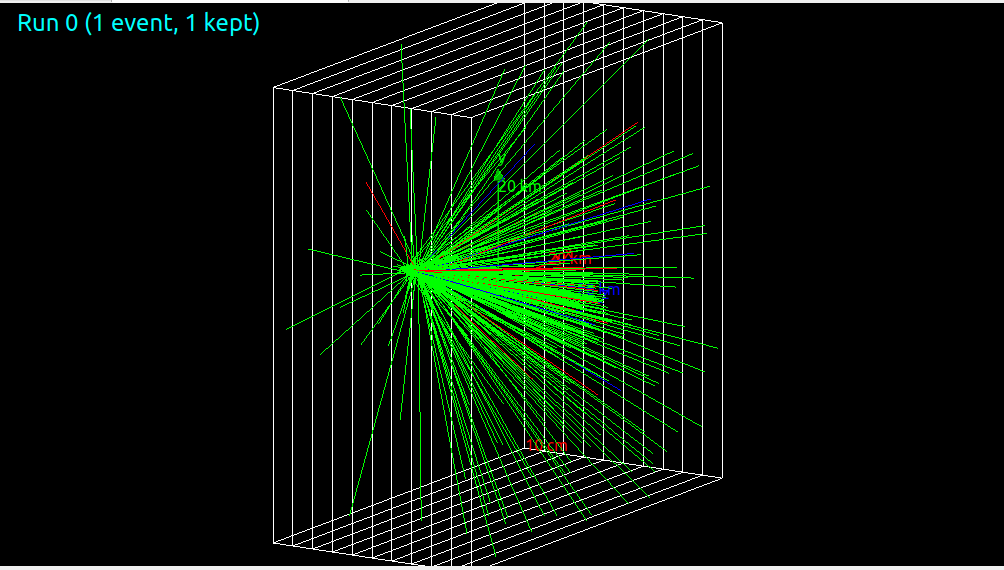
\includegraphics[scale=0.2]{Chapters/DusulMeu.png}};
\end{tikzpicture}

\begin{tikzpicture}[overlay, remember picture]
\node[anchor=center, 
      xshift=-3.5cm, 
      yshift=-1.5cm] 
     at (current page.center) 
     {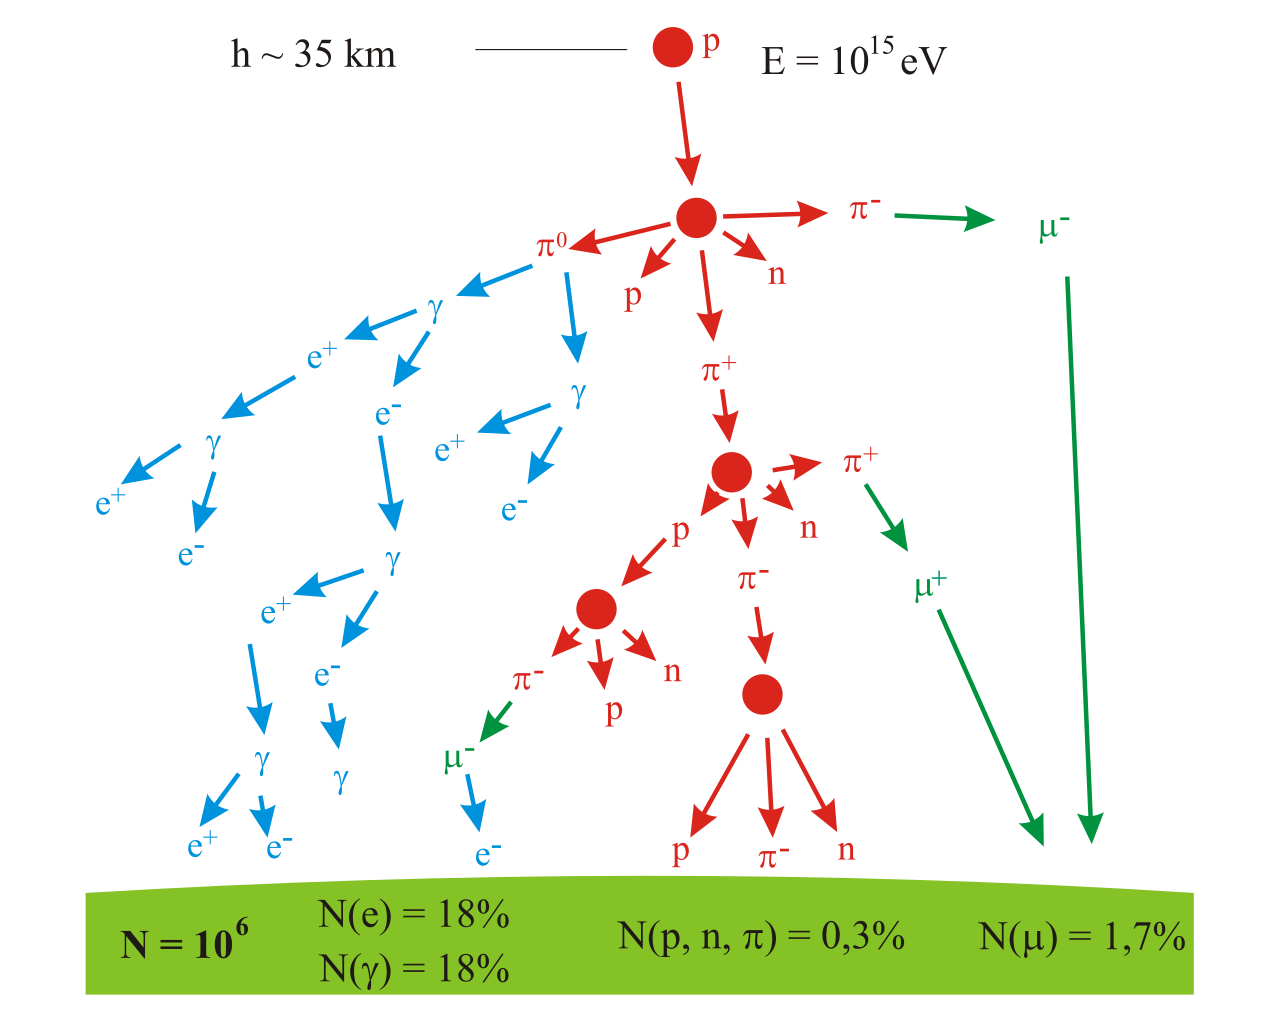
\includegraphics[scale=0.12]{Chapters/1280px-AirShower.png}};
\end{tikzpicture}

\end{frame}


\begin{frame}{\textbf{Jetul atmosferic - ramificații}}
\begin{tikzpicture}[overlay, remember picture]
\node[anchor=center, 
      xshift=0cm, 
      yshift=0cm] 
     at (current page.center) 
     {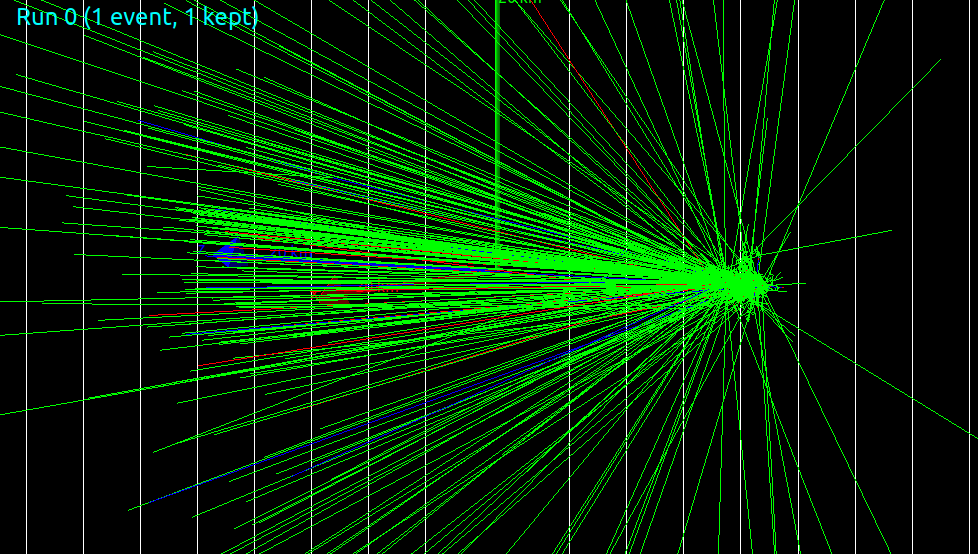
\includegraphics[scale=0.35]{Chapters/vertexuri.png}};
\end{tikzpicture}

\end{frame}

\begin{frame}{}
\begin{tikzpicture}[overlay, remember picture]
\node[anchor=center, 
      xshift=0cm, 
      yshift=0cm] 
     at (current page.center) 
     {\includegraphics[scale=0.22]{Chapters/Fluxul.png}};
\end{tikzpicture}

\end{frame}

%ultimul continut
\begin{frame}
\begin{tikzpicture}[overlay, remember picture]
\node[anchor=center, 
      xshift=0cm, 
      yshift=0cm] 
     at (current page.center) 
     {\includegraphics[scale=0.35]{Chapters/MicrosoftTeams-image (2).png}};
\end{tikzpicture}

\end{frame}


%final
\begin{frame}
\begin{tikzpicture}[overlay, remember picture]
\node[anchor=center, 
      xshift=0cm, 
      yshift=0cm] 
     at (current page.center) 
     {\includegraphics[scale=0.32]{Chapters/Showers-of-cosmic-ray-reactions-with-particles-of-the-atmosphere-Clo02.png}};
\end{tikzpicture}

\end{frame}

%sectiunea5
\section{\textbf{Aprecierea studentului.}}

\begin{frame}{\textbf{Propria părere despre activitatea desfășurată}}

\vspace{-0.5cm}
\makebox[1cm]{} \textit{\textbf{Pot afirma fără dubiu că sunt mulțumit de rezultatele obținute în raport cu totalitatea așteptărilor inițiale.}}
Activitatea mea s-a concentrat în special pe înțelegerea bazelor unui întreg ansamblu de instrumente soft relevate în studiul fenomenelor care implică interacțiunea particulelor cu materia și mai ales simularea comportării detectorilor de radiație \textbf{- HYPATIA + GEANT4}; 
.........................................................................................................................

\begin{enumerate}

\item[I)] \makebox[0.35cm]{} \textbf{ \textcolor{cyan}{ \textit{Mi-a plăcut enorm să cercetez diferite surse în vederea obținerii unor rezultate utile, edificând astfel logica programării abstracte în aplicații practice!}}}

\item[II)] \makebox[0.35cm]{} \textbf{ \textcolor{purple}{ \textit{ Un aspect negativ a constat în lipsa multor surse bine organizate  - vitale pentru simularea detectorului cu Ge și nu numai... }}}

\end{enumerate}

\end{frame}


%sectiunea6
\section{\textbf{Concluzii finale.}}

%skill-uri captate;
\begin{frame}{\textbf{Aspectele principale - ce am dobândit}}

\vspace{-0.25cm}
\textit{\textbf{\textcolor{red}{Deprinderile însușite:}}}


\begin{enumerate}

 \item[1)] \makebox[0.25cm]{} \textbf{ \textcolor{blue}{Folosirea și aprofundarea limbajului LaTeX( software-system pentru redactarea de documente tehnice.)}}
 \item[2)] \makebox[0.25cm]{} \textbf{ \textcolor{blue}{Manipularea sistemului de operare LINUX; instalarea și utilizarea unor pachete de programe marca UBUNTU.}} 
 \item[3)] \makebox[0.25cm]{} \textbf{ \textcolor{blue}{Detectarea și izolarea bosonilor Z, W și Higgs cu ajutorul softului HYPATIA- interpetarea datelor preluate la LHC-ATLAS.}} 
 \item[4)] \makebox[0.25cm]{} \textbf{ \textcolor{blue} {Folosirea unui soft de tip toolkit pentru programarea și simularea detectorilor.}} 
\item[5)] \makebox[0.25cm]{} \textbf{ \textcolor{blue}{Dobândirea unor cunoștințe suplimentare de programare în C++ și Python - depanarea de programe.}} 
\item[6)] \makebox[0.25cm]{} \textbf{ \textcolor{blue}{ Redactarea unor prezentări științifice despre subiectele tratate - structurarea conceptelor.}}



\end{enumerate}

\end{frame}



%ultimul frame - implicare vs valoare;
\begin{frame}{\textbf{Gradul de satisfacție și implicare în activitatea prestată}}

\vspace{-0.5cm}
\begin{itemize}
   
  \item[\ding{220}] \makebox[0.5cm]{} \textit{Activitățile prestate în debutul practicii \textbf{m-au impresionat într-un mod deosebit} - oferindu-mi în același timp o imagine de ansamblu mult mai clară asupra importanței laturii experimentale din sectorul Fizicii Nucleare.}
  
  \item[\ding{220}] \makebox[0.5cm]{} \textit{Dobândind diverse competențe în domeniul programării și simulării detectorilor am ajuns la un nivel profund de implicare} ce m-a făcut să pricep necesitatea unor resurse prețioase de programare.


 ------------------------------------------------------------------------------------------
  \item[\ding{227}]  \makebox[0.5cm]{} \textit{\textbf{\textcolor{violet}{În concluzie sunt încântat și plăcut surprins de ceea ce am reușit să fac pe baza multiplelor încercări repetate precum și a frecventelor "schimbări de paradigmă".}}}

\end{itemize}
\end{frame}

%final
\end{document}